\documentclass[twoside,a4paper,11pt]{memoir}
\usepackage{times}
\usepackage{pslatex}
\usepackage{url}
\usepackage{mscthesis}
\let\newfloat\undefined \usepackage{algorithmic} 
\usepackage{algorithm}
\usepackage{graphicx}
\usepackage{color}
\usepackage{hyperref}
\usepackage{adjustbox}
\usepackage{xspace}
\usepackage{enumitem}

\newcommand{\etal}{\emph{et al.}\xspace}
\newcommand\todo[1]{\textcolor{red}{TODO: #1}}

\def\chapterautorefname{Chapter} 
\def\sectionautorefname{Section} 
\def\subsectionautorefname{Section} 
% chktex-file 44
% chktex-file 41
% chktex-file 17

% \title{An in-depth case study on DDU}
% \title{DDU in Practice}
% \title{An exploration of DDU in practice}
\title{Exploring DDU in Practice}
\subtitle{Master's Thesis}

\author{Aaron Ang}
\authoremail{\url{a.w.z.ang@student.tudelft.nl}}
\birthplace{Amstelveen, The Netherlands}
\studentid{4139194}

\company{

\includegraphics[height=1.3cm]{figures/parc_logo.png}\\
PARC, a Xerox company\\
3333 Coyote Hill Road\\
Palo Alto, CA 94304\\
\url{www.parc.com}
}

\chair{Prof.\ Dr.\ A. van Deursen, Faculty EEMCS, TU Delft}
\supervisor{Prof.\ Dr.\ A. van Deursen, Faculty EEMCS, TU Delft}
\externalsupervisor{Dr.\ R. Maranhao, University of Lisbon}

\setcounter{tocdepth}{1}
\setsecnumdepth{subsection}
\maxsecnumdepth{subsection}

\begin{document}

\frontmatter
\thispagestyle{empty}
\maketitle
\makeformaltitlepages{TODO}

\chapter{Preface}%
\label{ch:preface}

TODO

\vspace{1cm}
\begin{flushright}
\theauthor%

Delft, The Netherlands

\today%
\end{flushright}

\cleardoublepage\tableofcontents
\cleardoublepage\listoffigures
\cleardoublepage\mainmatter%

\chapter{Introduction}%
\label{ch:introduction}
Software systems are complex and error-prone, likely to expose failures to the end user.
When a failure occurs, the developer has to debug the system to eliminate the failure.
This debugging process can be described in three phases~\cite{Parnin:2011:ADT:2001420.2001445}.
In the first phase, the developer has to pinpoint the fault, also known as the root cause, in code that causes the failure.
In the second phase, the developer has to develop an understanding of the root cause and its context.
Finally, in the third phase, the developer has to implement a patch that corrects the behavior of the system.
This process is time-consuming and can account for 30\% to 90\% of the software development cycle~\cite{robbins2003debugging, beizer2003software, britton2013reversible}.

Traditionally, developers use four different approaches to debug a software system, namely program logging, assertions, breakpoints and profiling~\cite{wong2016survey}.
Program logging is the act of inserting \emph{print} statements in the code to observe program state information during execution.
Assertions are constraints that can be added to a program that have to evaluate to true during execution time.
Breakpoints allow the developer to pause the software system during execution, and observe and modify variable values.
Profiling is used to perform runtime analysis and collect metrics on, for example, execution speed and memory usage.
These techniques provide an intuitive approach to localize the root cause of a failure, but, as one might expect, are less effective in the massive size and scale of software systems today.

Therefore, in the last decades a lot of research has been performed on improving and developing \emph{advanced} fault localization techniques~\cite{wong2016survey} such that they are applicable to the software systems of today.
A prominent fault localization technique is spectrum-based fault localization (SBFL).
SBFL techniques pinpoint faults in code based on execution information of a program, also known as a program spectrum~\cite{reps1997use}.
The output of SBFL techniques is a list of components, e.g.\ statements, branches or methods, ranked by their fault probability, allowing the developer to investigate the suspicious components consecutively.
Intuitively, if a statement is executed primarily during failed executions, then this statement might be assigned a higher suspiciousness score.
Similarly, if a statement is executed primarily during successful executions, then this statement might be assigned a lower suspiciousness score.
Ultimately, if the diagnostic performance of an SBFL technique is high, it means that the faulty component is ranked high in the diagnostic report, allowing the developer to spend less time on locating the root cause.

While SBFL techniques show promising results for debugging purposes, there are still aspects that prevent SBFL techniques from being used in practice.
First, in one of the pioneering user studies performed by Parnin and Orso~\cite{Parnin:2011:ADT:2001420.2001445}, the authors show that several assumptions made by SBFL techniques do not hold in practice.
For example, the authors find no evidence that the effectiveness of SBFL techniques is affected by the rank of the faulty statement.
Second, the diagnostic performance of SBFL techniques relies on the quality of the test suite.
SBFL techniques cannot accurately pinpoint a fault with a single failing test that covers multiple components.
However, if the test suite consists of many tests with different coverage patterns, then SBFL is able to pinpoint the fault more accurately because it can indict or exonerate components more precisely with more evidence, i.e.\ more execution traces.

The quality of test suites is commonly measured using an adequacy metric that focuses on error detection like statement coverage, branch coverage, method coverage.
However, these metrics do not necessarily enforce the quality of a test suite with respect to diagnosability --- the property of faults to be easily and precisely located~\cite{730889}.
For example, one could obtain a high test coverage (90\%) with a relative small number of tests that each covers a big part of the codebase.
In this case, when a test fails due to a fault, it is potentially difficult for SBFL techniques to pinpoint the root cause accurately due to a failing test that covers a large portion of the codebase and a small number of tests, lowering the possibility for SBFL techniques to accurately indict or exonerate components from being faulty.

For this reason, Perez \etal~\cite{DBLP:conf/icse/PerezAD17} propose a new metric, called DDU, to quantify the diagnosability of test suites as opposed to adequacy metrics that focus on error detection.
The objective of optimizing test suites with respect to DDU is to improve the diagnosability of test suites and consequently improve the diagnostic performance of SBFL techniques.
The authors have shown empirical evidence that optimizing a test suite with respect to DDU improves the diagnostic performance of SBFL by 34\% compared to a test suite that is optimized with respect to branch coverage.

\section{Problem Definition}%
\label{sec:problem_definition}
However, DDU is not yet usable in practice.
Currently, when the DDU is computed for a given test suite, its value lies in the domain \([ 0, 1 ]\), where \(0\) suggests that the test suite's diagnosability is low, and \(1\) suggests that the test suite's diagnosability is high.
The problem with this value is that the developer does not know how to extend or update the test suite given a DDU value.
For example, when the test suite's DDU is equal to \(0.1\), it is impossible for the developer to know what tests to write to improve the DDU\@.
In other words, time spent on software debugging (using SBFL techniques) cannot be reduced using DDU because its practical implications are unclear to the developer.

\section{Goal}
Although DDU is currently not usable in practice, Perez \etal~\cite{DBLP:conf/icse/PerezAD17} have shown that optimizing a test suite with respect to DDU can yield a 34\% gain in diagnostic performance using SBFL under constraint conditions\@.
Having a test suite with a high diagnosability could possibly reduce the time spent debugging because the fault is easier to pinpoint using SBFL techniques.
Therefore, the goal of this thesis is to explore how DDU behaves in practice and to find ways to make DDU usable in practice.
In other words, we explore possibilities to convey DDU to the developer such that the developer knows what kind of tests to write to improve the system's diagnosability.

\section{Structure of Report}
The structure of this report is as follows.
In \Cref{ch:background}, we explain the relevant topics to understand this study, like spectrum-based fault localization, spectrum-based reasoning, wasted effort, diagnosability assessment metrics and DDU\@.
In \Cref{ch:research_questions}, we formalize the research questions and explain the motivation behind them.
Then, in \Cref{ch:rq1,ch:rq2,ch:rq3}, we discuss the experimental design and results to answer the research questions.
Finally, in \Cref{ch:conclusion}, we conclude this study with a summary and recommendations for future work.

\chapter{Background}%
\label{ch:background}

In this chapter, we discuss topics that are relevant to understanding this study.
First, we discuss spectrum-based fault localization and spectrum-based reasoning, which are used in the experiments to perform fault diagnosis.
Second, we discuss the metric used to evaluate the diagnostic performance of spectrum-based fault localization techniques.
Then, we explain the definition of diagnosability and diagnosability assessment metrics.
Finally, we discuss how DDU was evaluated in the study that proposed DDU\@.

\section{Spectrum-Based Fault Localization (SBFL)}
In spectrum-based fault localization, we define a finite set \(\mathcal{C} = \langle c_1, c_2, \ldots, c_M \rangle \) of \(M\) system components, and a finite set \(\mathcal{T} = \langle t_1, t_2, \ldots, t_N \rangle \) of \(N\) system transactions, i.e.\ test executions.
The outcomes of all system tests are defined as an error vector \(e = \langle e_1, e_2, \ldots, e_N \rangle \), where \(e_i = 1 \) indicates that test \(t_i \) has failed and \(e_i = 0 \) indicates that test \(t_i \) has passed.
To keep track of which system components were executed during which test execution, we construct a \(N \times M \) activity matrix \(\mathcal{A} \), where \(\mathcal{A}_{ij} = 1 \) indicates that component \(c_j \) was exercised during test \(t_i \).
The pair \((\mathcal{A}, e) \) is also known as a program spectrum, which was first coined by Reps \etal~cite{reps1997use}.

Given the program spectrum, SBFL techniques compute the suspiciousness scores of system components, resulting in a diagnostic report, which is a list of components ranked by their fault probability.
The fault probabiliy is often computed using a similarity coefficient~\cite{Jones_visualizationfor, 4041886, Naish:2011:MSS:2000791.2000795, 6651713, 5772029, ERICWONG2010188, 6058639}.
Intuitively, the similarity coefficient indicates the similarity between the component's activity and the error vector.
When a component is more frequently exercised by test executions that fail, then the component is more likely to be faulty.
Conversely, when a component is more frequently exercised by test executions that pass, then the component is more likely to be healthy.


\section{Spectrum-Based Reasoning (SBR)}%
\label{sec:sbr}
Spectrum-based reasoning distinguishes itself from SBFL techniques by leveraging a reasoning framework.
The diagnostic report is generated by reasoning about the program spectrum instead of using a so-called similarity coefficient.
The two main phases of SBR are candidate generation and candidate ranking:
\begin{enumerate}
  \item In the candidate generation phase, a set \(\mathcal{D} = \langle d_1, d_2, \dots, d_k \rangle \) is constructed using a minimal hitting set (MHS) algorithm to cover all failing transactions, where each candidate \(d_i \) is a subset of \(\mathcal{C} \).
  An MHS algorithm is used to prevent generating a large number of diagnostic candidates~\cite{Abreu:2009:SMF:1747491.1747511}.

  \item In the candidate ranking phase, the fault probability for each candidate \(d_i \) is computed using the Naive Bayes rule~\cite{Abreu:2009:SMF:1747491.1747511}:
  \begin{equation}
    P(d_i | (\mathcal{A}, e)) = P(d_i) \cdot \prod_{j \in 1..N} \frac{P((\mathcal{A}_j, e_j) | d_i)}{P(\mathcal{A}_j)}
  \end{equation}
  \(P(d_i) \) is the prior probability, i.e.\ the probability that \(d_i \) is faulty without any evidence.
  \(P(\mathcal{A}_j) \) is a normalizing term that is identical for all candidates.
  \(P((\mathcal{A}_j, e_j) | d_i) \) changes the prior probability with every new observation from the program spectrum.
  This term can be computed using maximum likelihood estimation.
\end{enumerate}

In the experiments of this study, we make use of \textsc{Staccato}~\cite{conf/sara/AbreuG09} to generate candidates, and \textsc{Barinel}~\cite{Abreu:2009:SMF:1747491.1747511}, which implements spectrum-based reasoning, to rank candidates, i.e.\ perform software fault localization.

\section{Evaluation of Diagnosis}
Presently, cost of diagnosis \(C_d \) and wasted effort~\cite{Abreu:2009:SMF:1747491.1747511, 7390282, 6693085, Steimann:2013:TVV:2483760.2483767, DBLP:conf/icse/PerezAD17} are the most prevalent evaluation metrics for software fault localization (SFL) techniques.
In essence, \(C_d \) computes the number of components that have to be inspected before the actual fault is investigated in the diagnostic report.
When \(C_d = 0 \), it indicates that the actual fault is ranked first in the diagnostic report and, therefore, no effort is wasted investigating diagnosed components that are non-faulty.
Wasted effort (or effort) is the cost of diagnosis normalized by the number of components in the diagnostic report.

Both evaluation metrics assume \emph{perfect bug understanding}, which has been pointed out by Parnin and Orso~\cite{Parnin:2011:ADT:2001420.2001445} as a non-realistic assumption.
However, cost of diagnosis and effort serve as an objective evaluation metric that can be used for comparison and therefore will also be used in this study.

\section{Diagnosability}
Diagnosability is the property of faults to be easily and precisely located~\cite{730889}.
In other words, given that a fault exists in a software system, if the test suite's diagnosability is high and we would perform SFL using an automated debugging technique, then the faulty component would be ranked high in the diagnostic report, resulting in a low wasted effort.
On the contrary, if the test suite's diagnosability is low and we would perform SFL using an automated debugging technique, then the faulty component would be ranked low in the diagnostic report, resulting in a high wasted effort.

\section{Diagnosability Metric: Entropy}
The optimal diagnosability is achieved by having an exhaustive test suite that would exercise any combination of software components.
This way, any fault, whether it involves a single component or multiple components, can be diagnosed using an automated debugging technique with 100\% accuracy.
Perez \etal~\cite{DBLP:conf/icse/PerezAD17} find that Shannon's entropy accurately captures the test suite's exhaustiveness:
\begin{equation}
  H(T) = - \sum_i P(t_i) \cdot \log_2(P(t_i))
\end{equation}
where \(T \) is the set of unique test activities, and \(P(t_i) \) is the probability of test activity \(t_i \) occuring in the activity matrix.
The optimal entropy for a system with \(M \) components is \(M \) shannons, and therefore we can compute the normalized entropy \(\frac{H(T)}{M} \).
SBFL techniques are able to diagnose faults with 100\% accuracy when \(\frac{H(T)}{M} = 1.0 \).

However, an optimal normalized entropy would require \(2^M -1 \) tests, which is difficult to achieve in practice.
First, not all activity patterns can be generated from tests due to software topology, e.g.\ a basic block consisting of several statements --- these statements will always be executed together, and therefore on a statement granularity it is not possible to achieve optimal entropy, see \Cref{lst:topology}.
Second, systems of today can consist of millions of lines of code and would therefore require a non-realistic amount of effort to write the tests.\\
\begin{minipage}{\linewidth}
\begin{lstlisting}[caption={Lines 4 - 9 will always be executed together and therefore no optimal entropy can be achieved on a statement granularity. Same holds for lines 11 - 14.},label={lst:topology}]
public FieldRotation(final T q0, final T q1, final T q2, final T q3, final boolean needsNormalization) {
    if (needsNormalization) {
        // normalization preprocessing
        final T inv =
                q0.multiply(q0).add(q1.multiply(q1)).add(q2.multiply(q2)).add(q3.multiply(q3)).sqrt().reciprocal();
        this.q0 = inv.multiply(q0);
        this.q1 = inv.multiply(q1);
        this.q2 = inv.multiply(q2);
        this.q3 = inv.multiply(q3);
    } else {
        this.q0 = q0;
        this.q1 = q1;
        this.q2 = q2;
        this.q3 = q3;
    }
}
\end{lstlisting}
\end{minipage}

\section{Diagnosability Metric: DDU}
To elevate the problem with entropy, Perez \etal~\cite{DBLP:conf/icse/PerezAD17} propose a new diagnosability metric: DDU\@.
DDU combines three diagnosability metrics that capture characteristics of the activity matrix, namely normalized density, diversity, and uniqueness.

\subsection{Normalized Density}
Prior work~\cite{5954476} has used density to assess the diagnosability of the activity matrix:
\begin{equation}
  \rho = \frac{\sum_{i,j}\mathcal{A}_{ij}}{N \cdot M}
\end{equation}
Gonz\`ales-Sanchez \etal~\cite{5954476} show by induction that the optimal density is obtained when \(\rho = 0.5 \).
For DDU, Perez \etal~\cite{DBLP:conf/icse/PerezAD17} propose a normalized density \(\rho' \) where its optimal value is 1.0 instead of 0.5:
\begin{equation}
  \rho' = 1 - | 1 - 2 \rho |
\end{equation}
An optimal value for normalized density can be obtained without improving the diagnosability.
For exampe, in \Cref{subfig:no_diversity}, we observe that four tests (\(t_1\), \(t_2\), \(t_3\), \(t_4\)) have identical activation patterns, i.e.\ identical rows.
Assuming that the tests are deterministic, if component \(c_1\) is faulty, then all four tests will fail and therefore tests \(t_2\), \(t_3\), \(t_4\) do not add any value from the diagnosability perspective, i.e.\ tests \(t_2\), \(t_3\), \(t_4\) do not help SBFL techniques to further indict or exonerate components.
For this reason, Perez \etal~\cite{DBLP:conf/icse/PerezAD17} propose two enhancements: diversity and uniqueness.

\subsection{Diversity}
\begin{figure*}
    \centering
    \begin{subfigure}[b]{0.49\linewidth}
        \centering
        \begin{tabular}{c|cccc}
          & \(c_1 \) & \(c_2 \) & \(c_3 \) & \(c_4 \)     \\ \hline
          \(t_1 \) & 1 & 1 & 0 & 0 \\
          \(t_2 \) & 1 & 1 & 0 & 0 \\
          \(t_3 \) & 1 & 1 & 0 & 0 \\
          \(t_4 \) & 1 & 1 & 0 & 0 \\
        \end{tabular}
        \caption{No test diversity. \(\rho' = 1.0 \), \(\mathcal{G}=0.0 \)}%
        \label{subfig:no_diversity}
    \end{subfigure}
    \hfill
    \begin{subfigure}[b]{0.49\linewidth}
        \centering
        \begin{tabular}{c|cccc}
          & \(c_1 \) & \(c_2 \) & \(c_3 \) & \(c_4 \)     \\ \hline
          \(t_1 \) & 1 & 1 & 0 & 0 \\
          \(t_2 \) & 0 & 0 & 1 & 1 \\
          \(t_3 \) & 1 & 1 & 1 & 0 \\
          \(t_4 \) & 0 & 0 & 0 & 1 \\
        \end{tabular}
        \caption{Component ambiguity. \(\rho' = 1.0 \), \(\mathcal{G}=1.0 \), \(\mathcal{U}=0.75 \) }%
        \label{subfig:ambiguity}
    \end{subfigure}
    \vskip\baselineskip%
    \begin{subfigure}[b]{0.49\linewidth}
        \centering
        \begin{tabular}{c|cccc}
          & \(c_1 \) & \(c_2 \) & \(c_3 \) & \(c_4 \)     \\ \hline
          \(t_1 \) & 1 & 1 & 0 & 0 \\
          \(t_2 \) & 0 & 1 & 1 & 0 \\
          \(t_3 \) & 1 & 0 & 1 & 1 \\
          \(t_4 \) & 0 & 0 & 0 & 1 \\
        \end{tabular}
        \caption{No component ambiguity. \(\rho' = 1.0 \), \(\mathcal{G}=1.0 \), \(\mathcal{U}=1.0 \)}%
        \label{subfig:no_ambiguity}
    \end{subfigure}
    \caption{The effect of diversity and uniqueness on diagnosability.}%
    \label{fig:diversity_ambiguity}
\end{figure*}

The first enhancement to normalized density is diversity, which ensures test diversity among the activity matrix's rows.
The test diversity is low when the test suite consists of many tests that have identical activity patterns, i.e.\ rows.
Conversely, the test diversity is high when the test suite consists of many tests that have distinct activity patterns.

Perez \etal~\cite{DBLP:conf/icse/PerezAD17} use the Gini-Simpson index \(\mathcal{G} \)~\cite{OIK:OIK14714} to capture test diversity:
\begin{equation}
  \mathcal{G} = 1 - \frac{\sum_{i \in 1..|G|} |g_i| \cdot (|g_i| - 1)}{N \cdot (N - 1)}
\end{equation}
where \(G = \langle g_1, \dots, g_k \rangle \) is the set of ambiguity groups among the rows, \(|g_i |\) is the number of test with identical activation patterns, and \(N \) is the number of tests.
To clarify how this formula is used, we give two examples.
In \Cref{subfig:no_diversity}, there is one ambiguity group \(g_1 = \langle t_1, t_2, t_3, t_4 \rangle \), resulting in \(\mathcal{G} = 1 - \frac{4 \cdot 3}{4 \cdot 3} = 0.0\).
In \Cref{subfig:ambiguity}, there are four ambiguity groups, \(g_1 = \langle t_1 \rangle, g_2 = \langle t_2 \rangle, g_3 = \langle t_3 \rangle, g_4 = \langle t_4 \rangle \), resulting in \(\mathcal{G} = 1 - \frac{1 \cdot 0 + 1 \cdot 0 + 1 \cdot 0 + 1 \cdot 0}{4 \cdot 3} = 1.0\).
As we can observe in \Cref{subfig:ambiguity}, when optimizing the activity matrix for test diversity, the shortcoming of normalized density, shown in \Cref{subfig:no_diversity}, is mitigated.

\subsection{Uniqueness}
The second enhancement to normalized density is uniqueness, which controls for the number of ambiguity groups among the activity matrix's columns.
An ambiguity group is a set of components that have identical activation patterns across the test suite, i.e.\ identical columns in the activity matrix.
Component ambiguity is undesirable because it prevents SBR from updating the fault probabilities of the individual components in the ambiguity group, resulting in a less accurate diagnosis.
If test suite's uniqueness is low, then many components in the activity matrix have identical activity patterns, i.e.\ components are involved in the same test cases.
Conversely, if the test suite's uniqueness is high, then many components in the activity matrix have distinct activity patterns.

Given the set of component ambiguity groups \(G = \langle g_1, \dots, g_l \rangle \), then the test suite's uniqueness is computed as follows:
\begin{equation}
  \label{eq:uniqueness}
  \mathcal{U} = \frac{|G|}{M}
\end{equation}
where \(|G|\) is the number of ambiguity groups and \(M\) is the number of components, i.e.\ columns.
To clarify how this formula is used, we give two examples.
In \Cref{subfig:ambiguity}, there are 3 ambiguity groups: \( g_1 = \langle c_1, c_2 \rangle \), \( g_2 = \langle c_3 \rangle \), \( g_3 = \langle c_4 \rangle \), resulting in \( \mathcal{U} = \frac{3}{4} = 0.75 \).
In \Cref{subfig:no_ambiguity}, there are 4 ambiguity groups: \( g_1 = \langle c_1 \rangle \), \( g_2 = \langle c_2 \rangle \), \( g_3 = \langle c_3 \rangle \), \( g_4 = \langle c_4 \rangle \), resulting in \( \mathcal{U} = \frac{4}{4} = 1 \)

We observe in \Cref{subfig:ambiguity} that optimizing the test suite with respect to normalized density and diversity can still result in component ambiguity groups, namely \(\langle c_1, c_2 \rangle \).
When optimizing the test suite with respect to normalized density, diversity and uniqueness, we observe in \Cref{subfig:no_ambiguity} that there are no identical test activity patterns and no ambiguity groups, which results in a better diagnosability.

\subsection{Combined}
The DDU combines normalized density, diversity, and uniqueness as follows:
\begin{equation}
 DDU = normalized\ density \cdot diversity \cdot uniqueness
\end{equation}
If \(DDU = 1 \), then the test suite's diagnosability is high.
Vice versa, if \(DDU = 0 \), then the test suite's diagnosability is low.
Perez \etal~\cite{DBLP:conf/icse/PerezAD17} have shown in an experiment that optimizing a test suite with respect to DDU yields a 34\% diagnostic performance compared to a test suite optimized for branch coverage.

\section{Evaluation of DDU}
In the study that proposed DDU, Perez \etal~\cite{DBLP:conf/icse/PerezAD17} performed two experiments to answer three research questions:
\begin{enumerate}[noitemsep]
    \item [\textbf{RQ1}] Is the DDU metric more accurate than the state-of-the-art in diagnosability assessment?
    \item [\textbf{RQ2}] How close does the DDU metric come to the (ideal yet intractable) full entropy?
    \item [\textbf{RQ3}] Does optimizing a test-suite with regard to DDU result in better diagnosability than optimizing adequacy metrics such as branch-coverage in traditional scenarios?
\end{enumerate}
The goal of their study was to evaluate how DDU compares with the existing metrics: entropy, density, uniqueness, and branch coverage.

The empirical evaluation leveraged a test-generation approach using \textsc{EvoSuite}\footnote{\url{http://www.evosuite.org/}}, which employs search-based software testing approaches.
\textsc{EvoSuite} generates tests to minimize a fitness function using genetic algorithms.
In essence, the fitness function is a measure that indicates the distance between a given solution and the optimal solution.
For example, in the case of DDU, the optimal solution is \(\emph{DDU} = 1\) and, therefore, \textsc{EvoSuite} generates tests to minimize the differene between the current test suite's DDU value and the optimal DDU value.

To answer \textbf{RQ1} and \textbf{RQ2}, the authors generated test suites for each class in the open source projects Commons Codec, Commons Compress, Commons Math and JodaTime that are optimized with respect to DDU, branch coverage, entropy, density and uniqueness.
For each test suite, the activity matrix is constructed and, subsequently, the error vector is generated by artificially injecting faults --- single-component and two-component faults.
Then, given these program spectra, on each program spectrum SBR is performend to generate a diagnostic report.
Finally, the wasted effort is computed for each diagnostic report, which enables the authors to compare the diagnostic performance of DDU against the diagnostic performance of branch coverage, entropy, density, uniqueness.

To answer \textbf{RQ3}, the authors make use of the \textsc{Defects4J} database, which contains 357 real software bugs from 5 open source projects.
The database contains a faulty and fixed software version for each bug.
For each bug, the authors generate two test suites for the fixed software version --- one test suite that optimizes DDU and one that optimizes branch coverage.
Then, instead of artificially injecting faults, the authors run the generated test suite against the faulty software version and collect the program spectrum.
Subsequently, SBR is performed on the collected program spectra, enabling the comparison between DDU and branch coverage.

\chapter{Research Questions}%
\label{ch:research_questions}
Ideally, we would like to propose an intuitive approach that allows developers to use DDU in their software development cycle.
However, there has been no study yet on DDU that investigates how it actually behaves in practice.
For this reason, the goal of this study is to explore how DDU behaves in practice and to find ways to make DDU usable in practice.
To achieve this goal, we define three research questions.

\begin{framed}
\noindent
\textbf{RQ1:} How do normalized density, diversity, uniqueness, and DDU vary in practice?
\end{framed}
To be able to propose an intuitive approach that allows developers to use DDU in practie, we first need to understand how the metrics vary in practice.
By analyzing how these metrics perform in practice, we are able to propose improvements for DDU, and potentially propose an approach that enables DDU in practice.

\begin{framed}
\noindent
\textbf{RQ2:} What is the relation between normalized density, diversity, uniqueness, and DDU and diagnosability?
\end{framed}
In Perez \etal's work~\cite{DBLP:conf/icse/PerezAD17}, the authors show that generating tests with respect to DDU yields a 34\% diagnostic performance compared to a test suite optimized for branch coverage.
However, this does necessarily imply that DDU is strongly correlated with diagnosability.
Therefore, we would like to validate that DDU and diagnosability are strongly correlated, i.e.\ the higher DDU, the better the diagnosability, and vice versa.
This question is important to answer because DDU was proposed as a metric to quantify the diagnosability.

\begin{framed}
\noindent
\textbf{RQ3:} What is the relation between density, diversity, uniqueness, and DDU and test coverage?
\end{framed}
The intention of test coverage is to optimize for error detection.
Perez \etal~\cite{DBLP:conf/icse/PerezAD17} propose DDU as a complementary metric to test coverage because DDU is meant to capture the diagnosability and not error detection.
However, if there is a strong correlation between DDU and test coverage, then DDU could possibly replace test coverage as a test adequacy metric, which is a use case that the authors have not thought of.
Furthermore, assuming that DDU is strongly correlated with diagnosability and test coverage is representative for error detection, answering this research question will give us a better understanding on the relation between diagnosability and error detection, and could give us insight in how DDU and test coverage can be used together in practice.

\chapter{DDU in Practice}%
\label{ch:rq1}
\begin{framed}
\noindent
\textbf{RQ1:} How do normalized density, diversity, uniqueness, and DDU vary in practice?
\end{framed}
In this chapter, the goal is to obtain a better intuition on what common values are for density, diversity, uniquness, and DDU by analyzing open source projects hosted on GitHub.
First, we take a look at the distributions of normalized density, diversity, uniqueness, and DDU\@.
Second, we give examples of classes that have a low or high value for any of the diagnosability metrics and analyze why these components have either a low or high value by investigating the class' test suite.
Finally, we conclude this chapter with a list of observations.

\section{Approach}
To get a better understanding of how the values vary for normalized density, diversity, uniqueness, and DDU, we use \texttt{ddu-maven-plugin}\footnote{\url{https://github.com/aperez/ddu-maven-plugin}}, developed by Perez, to instrument Java code and construct the activity matrix.
Once we obtain the activity matrices, we analyze the data using multiple Python scripts\footnote{\url{https://github.com/aaronang/ddu}}.
With these two tools we collect data such as density, normalized density, diversity, uniqueness, DDU, and the activity matrix.

Then, we analyze the collected data and show examples to illustrate how DDU and its individual terms vary as a consequence to particular kinds of tests or testing strategies.
We are interested in what kinds of testing approaches result in a high or low value.

Note that \texttt{ddu-maven-plugin} is able to instrument the code for three different granularity levels, namely statements, branches, and methods.
By default \texttt{ddu-maven\-plugin} uses the method level granularity.
In this study, we make use of the same granularity used in the study performed by Perez \etal~\cite{DBLP:conf/icse/PerezAD17}, namely branch granularity.

\section{Selection}
The selection of open source projects is done according to the following criteria.
\begin{itemize}[noitemsep]
  \item \emph{The project must have an executable test suite.}
  To compute the DDU for a software project, we must construct an activity matrix.
  The activity matrix is constructed by running the test suite and instrumenting the code to keep track of which components are executed during a program execution.
  Since we are interested in the activity matrix \(\mathcal{A}\), we do not care if a test suite has failing tests.
  A project meets this criterion as long as the test suite executes and does not crash.

  \item \emph{The project must use Apache Maven, a software project management and comprehension tool.}
  The current tool that instruments the code to construct the activity matrix is implemented as a Maven plugin.
  Note that the current Maven plugin does not work for all Maven projects and, therefore, only projects that can be analyzed with this plugin are used.
\end{itemize}

Based on these requirements, we choose the following open source projects.
\begin{itemize}[noitemsep]
    % \item Commons CSV\footnote{\url{https://github.com/apache/commons-csv}}: a library that provides a simple interface for reading and writing CSV files of various types.
    % \item Commons Text\footnote{\url{https://github.com/apache/commons-text}}: a library focused on algorithms working on strings.
    % \item Commons IO\footnote{\url{https://github.com/apache/commons-io}}: a library of utilities to assist with developing IO functionality.
    \item Commons Codec\footnote{\url{https://github.com/apache/commons-codec}}: a package that contains simple encoders and decoders for various formats such as Base64 and Hexadecimal.
    \item Commons Compress\footnote{\url{https://github.com/apache/commons-compress}}: an API for working with compression and archive formats.
    \item Commons Math\footnote{\url{https://github.com/apache/commons-math}}: a library of lightweight, self-contained mathematics and statistics components addressing the most common practical problems.
    \item Guice\footnote{\url{https://github.com/google/guice}}: a lightweight dependency injection framework for Java 6 and above.
    \item Jsoup\footnote{\url{https://github.com/jhy/jsoup}}: an API for extracting and manipulating data, using the best of DOM, CSS, and jquery-like methods.
\end{itemize}
Note that some of the projects are also used in Perez \etal's study~\cite{DBLP:conf/icse/PerezAD17}.
In \Cref{tab:project_statistics}, we show some statistics for each project.
The number of classes, methods, and lines were obtained by running the complete test suites in IntelliJ and collecting the coverage report.
The number of branches was obtained by running the complete test suite while the \textsc{ddu-maven-plugin} instruments the code using the branch granularity and consequently counting the number of components in the program spectrum.
% project_name,number_of_classes,number_of_methods,number_of_branches,number_of_lines
% Commons Codec,87,743,2901,3827
% Commons Compress,261,2143,8650,12182
% Commons Math,977,7406,33614,45004
% Guice,332,2039,9134,7102
% Jsoup,232,1343,5088,6875

% Please add the following required packages to your document preamble:
% \usepackage[table,xcdraw]{xcolor}
% If you use beamer only pass "xcolor=table" option, i.e. \documentclass[xcolor=table]{beamer}
\begin{table}[]
\centering
\caption{Statistics of open source projects.}%
\label{tab:project_statistics}
\begin{tabular}{lllll}
    \toprule
    Subject          & Classes & Methods & Branches & Lines \\
    \rowcolor{Gray} 
    Commons Codec    & 87      & 743     & 2901     & 3827  \\
    Commons Compress & 261     & 2143    & 8650     & 12182 \\
    \rowcolor{Gray} 
    Commons Math     & 977     & 7406    & 33614    & 45004 \\
    Guice            & 332     & 2039    & 9134     & 7102  \\
    \rowcolor{Gray} 
    Jsoup            & 232     & 1343    & 5088     & 6875 \\
    \bottomrule
\end{tabular}
\end{table}

\section{Normalized Density}

In \autoref{fig:hist_normalized_density}, we show the distribution of normalized densities for all classes of the five open source projects mentioned before.
The average equals to 0.5145.
The peak for the interval [0, 0.1) is primarily caused by classes that are exercised by tests that involve all components.
In the interval [0, 0.1), 43 classes consist of only one branch.
A class with one branch will always have a density of 1.0 and therefore a normalized density of 0.

\begin{figure}
    \centering
    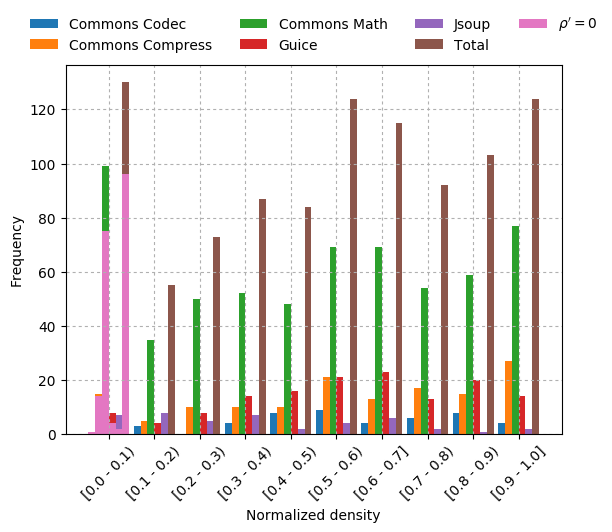
\includegraphics[width=\linewidth]{figures/grouped_barchart_density}
    \caption{Normalized density distribution.}%
    \label{fig:hist_normalized_density}
\end{figure}

The normalized density value is low when a class is tested by many tests that only cover a couple of branches, or covered by tests that involve all components.
For example, the class \texttt{ProvidesMethodScanner} has 35 branches and its partial activity matrix is shown in \Cref{tab:providesmethodscanner}, where the columns represent branches of \texttt{Provides\-Method\-Scanner}.
In the first row, we observe that the transaction \texttt{test\-Untargetted\-Binding} only hits one branch \(c_{23} \), indicated by a 1.
We observe that all transactions in the activity matrix have a similar coverage.
Since every transaction is only hitting a few components, the normalized density is low.
Moreover, \texttt{Provides\-Method\-Scanner} has 35 components and if a transaction only hits a few components, it results in the activity matrix to become sparse.

\begin{table}[]
\scriptsize
\centering
\caption{Partial activity matrix of the \texttt{com.google.\-inject.\-internal.\-Provides\-Method\-Scanner} class where \(\rho' = 0.111\).}%
\label{tab:providesmethodscanner}
\begin{tabular}{l|ccccccc}
transaction & \(c_1 \) & \dots & \(c_{22} \) & \(c_{23} \) & \(c_{24} \) & \dots & \(c_{35} \) \\ \hline
\texttt{BinderTest\#testUntargettedBinding} & 0 & \dots & 0 & 1 & 0 & \dots & 0 \\
\texttt{BinderTest\#testMissingDependency} & 0 & \dots & 0 & 1 & 0 & \dots & 0 \\
\texttt{BinderTest\#testProviderFromBinder} & 0 & \dots & 0 & 1 & 0 & \dots & 0 \\
\texttt{BinderTest\#testToStringOnBinderApi} & 0 & \dots & 0 & 1 & 0 & \dots & 0 \\
\texttt{BinderTest\#testUserReportedError} & 0 & \dots & 0 & 1 & 0 & \dots & 0 \\
\vdots & \vdots & \vdots & \vdots & \vdots & \vdots & \vdots & \vdots
\end{tabular}
\end{table}

\begin{table}[]
\scriptsize
\centering
\caption{Activity matrix of the \texttt{org.apache.commons.math4.fitting.leastsquares.CircleProblem} class where \(\rho' = 0\) because every transaction covers every component.}%
\label{tab:circleproblem}
\begin{tabular}{l|cccc}
transaction & \(c_1 \) & \(c_2 \) & \dots & \(c_{26} \) \\ \hline
\texttt{LevenbergMarquardtOptimizerTest\#testParameterValidator} & 1 & 1 & \dots & 1 \\
\texttt{LevenbergMarquardtOptimizerTest\#testCircleFitting2} & 1 & 1 & \dots & 1
\end{tabular}
\end{table}

In the activity matrix of \texttt{Circle\-Problem}, shown in \Cref{tab:circleproblem}, we observe a high density; all branches of \texttt{Circle\-Problem} are hit in every single test.
This results in a low normalized density: 0.0, because the density is high: 1.0.

Thus, ideally, to obtain a high value for the normalized density, we need a good balance between tests that cover many components and tests that cover a few.
In Commons Math, the \texttt{Elitistic\-List\-Population} class has a nearly optimal normalized density.
In its activity matrix, see \Cref{tab:elitistic}, we observe that there is a good balance between tests that cover a few components and tests that cover many components, resulting in a normalized density of 0.979.

\begin{table}[]
\scriptsize
\centering
\caption{Activity matrix of \texttt{org.apache.commons.math4.genetics.Elitistic\-List\-Population} where \(\rho' = 0.979\).}%
\label{tab:elitistic}
\begin{adjustbox}{center}
\begin{tabular}{l|llllllll}
transaction                                                       & \(c_1 \) & \(c_2 \) & \(c_3 \) & \(c_4 \) & \(c_5 \) & \(c_6 \) & \(c_7 \) & \(c_8 \) \\ \hline
\texttt{ElitisticListPopulationTest\#testChromosomeListConstructorTooLow}  & 1     & 0     & 0     & 1     & 0     & 0     & 0     & 0     \\
\texttt{ElitisticListPopulationTest\#testSetElitismRateTooLow}             & 1     & 0     & 0     & 1     & 0     & 0     & 1     & 0     \\
\texttt{ElitisticListPopulationTest\#testConstructorTooHigh}               & 1     & 0     & 0     & 1     & 0     & 0     & 0     & 0     \\
\texttt{ElitisticListPopulationTest\#testConstructorTooLow}                & 1     & 0     & 0     & 1     & 0     & 0     & 0     & 0     \\
\texttt{ElitisticListPopulationTest\#testSetElitismRateTooHigh}            & 1     & 0     & 0     & 1     & 0     & 0     & 1     & 0     \\
\texttt{ElitisticListPopulationTest\#testChromosomeListConstructorTooHigh} & 1     & 0     & 0     & 1     & 0     & 0     & 0     & 0     \\
\texttt{ElitisticListPopulationTest\#testSetElitismRate}                   & 1     & 0     & 0     & 0     & 0     & 1     & 1     & 0     \\
\texttt{ElitisticListPopulationTest\#testNextGeneration}                   & 1     & 1     & 1     & 0     & 1     & 1     & 1     & 1     \\
\texttt{FitnessCachingTest\#testFitnessCaching}                            & 1     & 1     & 1     & 0     & 1     & 1     & 1     & 1     \\
\texttt{GeneticAlgorithmTestBinary\#test}                                  & 1     & 1     & 1     & 0     & 1     & 1     & 1     & 1     \\
\texttt{GeneticAlgorithmTestPermutations\#test}                            & 1     & 1     & 1     & 0     & 1     & 1     & 1     & 1     \\
\texttt{TournamentSelectionTest\#testSelect}                               & 1     & 0     & 0     & 0     & 0     & 0     & 1     & 0
\end{tabular}
\end{adjustbox}
\end{table}

% In short, to obtain a good value for normalized density, a test suite should have a good balance between tests that cover a few components and tests that cover many components.

\section{Diversity}
In \Cref{fig:histogram_diversity}, the distribution of diversity of classes is shown.
The average is 0.588.
The peak for the interval [0, 0.1) occurs for various reasons.
The first reason is that there are 43 classes with only one method and therefore every row is identical, resulting in a diversity of 0.
The second reason is that for 52 classes there exists only one test, and in the current Python script the diversity defaults to 0 when there is only one test.
The third reason is that there are test suites where all the test cases have identical activity patterns.
In total there are 176 classes with a diversity of 0, where 36 classes only have one method, 45 classes only have one test, and 7 classes only have one method and one test.

\begin{figure}
    \centering
    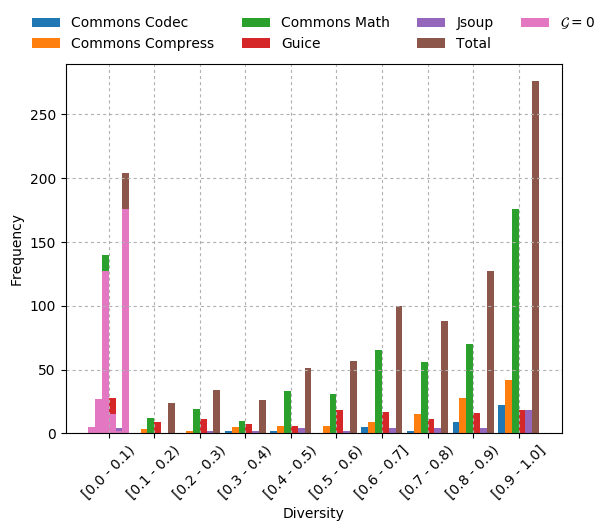
\includegraphics[width=\linewidth]{figures/grouped_barchart_diversity}
    \caption{Diversity distribution.}%
    \label{fig:histogram_diversity}
\end{figure}

Intuitively, the diversity has a low value when the number of identical transactions is high, i.e.\ identical rows in the activity matrix.
Conversely, the diversity is high when the number of identical transactions is low.

\begin{table}[]
\scriptsize
\centering
\caption{Partial activity matrix of \texttt{org.apache.commons.math4.analysis.function.Power} where \(\mathcal{G} = 0.077\).}%
\label{tab:power}
\begin{tabular}{l|ccc}
transaction & \(c_1 \) & \(c_2 \) & \(c_3 \) \\ \hline
\texttt{FunctionUtilsTest\#testFixingArguments} & 1 & 1 & 0 \\
\texttt{FunctionUtilsTest\#testMultiplyDifferentiable} & 1 & 0 & 1 \\
\texttt{FunctionUtilsTest\#testComposeDifferentiable} & 1 & 1 & 1 \\
\texttt{FunctionUtilsTest\#testCompose} & 1 & 1 & 0 \\
\texttt{FunctionUtilsTest\#testMultiply} & 1 & 1 & 0 \\
\texttt{ArrayRealVectorTest\#testMap} & 1 & 1 & 0 \\
\texttt{ArrayRealVectorTest\#testMapToSelf} & 1 & 1 & 0 \\
\texttt{RealVectorTest\#testMap} & 1 & 1 & 0 \\
\vdots & \vdots & \vdots & \vdots
\end{tabular}
\end{table}

In the partial activity matrix of \texttt{Power}, shown in \Cref{tab:power}, we observe that almost every transaction has an identical activity and therefore the diversity is low: 0.077.
Another reason for the low diversity of \texttt{Power} is that it is covered by 102 test cases, while there are only \(2^3 - 1 = 7 \) possible different tests for two components.
After 7 unique tests every additional test will have a negative effect on the diversity because it will share an identical activity with an existing test.

\begin{table}[]
\scriptsize
\centering
\caption{Activity matrix of \texttt{org.\-apache.\-commons.\-math4.\-ode.\-AbstractParameterizable} where \(\mathcal{G} = 0.933\).}%
\label{tab:abstractparameter}
\begin{adjustbox}{center}
\begin{tabular}{l|cccccccc}
 & \(c_1 \) & \(c_2 \) & \(c_3 \) & \(c_4 \) & \(c_5 \) & \(c_6 \) & \(c_7 \) & \(c_8 \) \\ \hline
\texttt{JacobianMatricesTest\#testHighAccuracyExternalDifferentiation} & 1 & 0 & 1 & 0 & 1 & 0 & 1 & 0 \\
\texttt{JacobianMatricesTest\#testAnalyticalDifferentiation} & 1 & 0 & 1 & 0 & 1 & 0 & 1 & 0 \\
\texttt{JacobianMatricesTest\#testInternalDifferentiation} & 0 & 0 & 0 & 0 & 1 & 0 & 1 & 0 \\
\texttt{JacobianMatricesTest\#testParameterizable} & 1 & 0 & 0 & 0 & 1 & 0 & 1 & 1 \\
\texttt{JacobianMatricesTest\#testWrongParameterName} & 0 & 0 & 1 & 1 & 1 & 1 & 0 & 1 \\
\texttt{JacobianMatricesTest\#testFinalResult} & 1 & 0 & 1 & 0 & 1 & 0 & 1 & 1
\end{tabular}
\end{adjustbox}
\end{table}

In the activity matrix of \texttt{Abstract\-Parameterizable}, shown in \Cref{tab:abstractparameter}, we observe that almost every transaction has a unique activity and therefore its diversity is high: 0.933.
Note that the diversity suffers when there are too many test cases, but does not suffer from a low number of test cases.

An interesting case for diversity is parameterized testing.
Although parameterized testing is a common practice to test different inputs for a unit, it can have a negative effect on the diversity if the various parameters chosen exhibit identical activity patterns.
An example is the class \texttt{Symmetric\-Gauss\-Integrator} with a diversity of 0.571, shown in \Cref{tab:hermite}.


\begin{table}[]
    \scriptsize
    \centering
    \caption{Partial activity matrix of \texttt{org.\-apache.\-commons.\-math4.\-analysis.\-integration.\-gauss.\-SymmetricGaussIntegrator}, where parameterized testing exhibits identical activity patterns.}%
    \label{tab:hermite}
    \begin{adjustbox}{center}
    \begin{tabular}{l|cccccccc}
     & \(c_1 \) & \(c_2 \) & \(c_3 \) & \(c_4 \) & \(c_5 \) & \(c_6 \) & \(c_7 \) & \(c_8 \) \\ \hline
    \texttt{HermiteParametricTest\#testAllMonomials[0]} & 0 & 1 & 1 & 0 & 0 & 0 & 0 & 0 \\
    \texttt{HermiteParametricTest\#testAllMonomials[1]} & 1 & 0 & 1 & 1 & 1 & 1 & 1 & 0 \\
    \texttt{HermiteParametricTest\#testAllMonomials[2]} & 1 & 0 & 1 & 1 & 1 & 1 & 1 & 1 \\
    \texttt{HermiteParametricTest\#testAllMonomials[3]} & 1 & 0 & 1 & 1 & 1 & 1 & 1 & 0 \\
    \texttt{HermiteParametricTest\#testAllMonomials[4]} & 1 & 0 & 1 & 1 & 1 & 1 & 1 & 1 \\
    \texttt{HermiteParametricTest\#testAllMonomials[5]} & 1 & 0 & 1 & 1 & 1 & 1 & 1 & 0 \\
    \vdots & \vdots & \vdots & \vdots & \vdots & \vdots & \vdots & \vdots & \vdots \\
    \texttt{HermiteParametricTest\#testAllMonomials[26]} & 1 & 0 & 1 & 1 & 1 & 1 & 1 & 1 \\
    \texttt{HermiteParametricTest\#testAllMonomials[27]} & 1 & 0 & 1 & 1 & 1 & 1 & 1 & 0 \\
    \texttt{HermiteParametricTest\#testAllMonomials[28]} & 1 & 0 & 1 & 1 & 1 & 1 & 1 & 1 \\
    \texttt{HermiteParametricTest\#testAllMonomials[29]} & 1 & 0 & 1 & 1 & 1 & 1 & 1 & 0
    \end{tabular}
    \end{adjustbox}
\end{table}


\section{Uniqueness}

The distribution of uniqueness of classes is shown in \Cref{fig:uniqueness}.
The average is 0.477.
The peak for the interval [0.9, 1.0] is partially caused by classes that only have one component; activity matrices that consist of one component always have a uniqueness of 1.0.
There are 130 classes that have a uniqueness of 1.0 and 43 out of the 130 classes only have one branch.

\begin{figure}
    \centering
    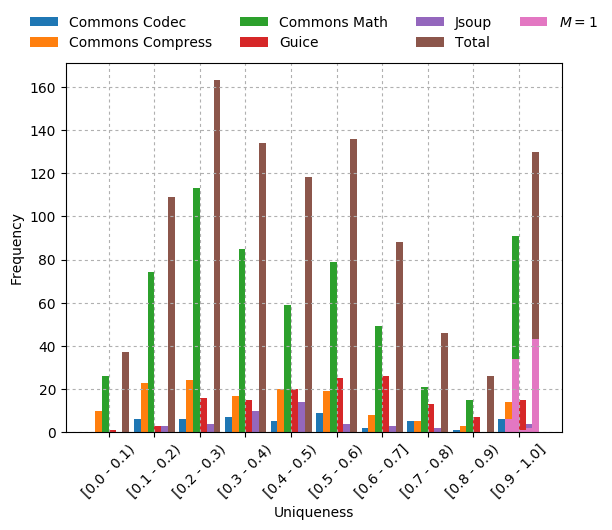
\includegraphics[width=\linewidth]{figures/grouped_barchart_uniqueness}
    \caption{Distribution of uniqueness.}%
    \label{fig:uniqueness}
\end{figure}

The uniqueness of a class is high when there is a high number of unique columns in the activity matrix.
Conversely, the uniqueness is low when there is a low number of unique columns in the activity matrix.

\begin{table}[]
\scriptsize
\centering
\caption{Activity matrix of \texttt{org.apache.commons.codec.digest.Crypt} where \(\mathcal{U} = 0.916\).}%
\label{tab:crypt}
\begin{adjustbox}{center}
\begin{tabular}{l|cccccccccccc}
 & \(c_1 \) & \(c_2 \) & \(c_3 \) & \(c_4 \) & \(c_5 \) & \(c_6 \) & \(c_7 \) & \(c_8 \) & \(c_9 \) & \(c_{10} \) & \(c_{11} \) & \(c_{12} \) \\ \hline
\texttt{CryptTest\#testDefaultCryptVariant} & 0 & 0 & 0 & 1 & 1 & 0 & 0 & 1 & 0 & 1 & 0 & 0 \\
\texttt{CryptTest\#testCryptWithEmptySalt} & 1 & 1 & 0 & 0 & 0 & 0 & 1 & 1 & 0 & 1 & 1 & 0 \\
\texttt{CryptTest\#testCryptWithBytes} & 0 & 1 & 1 & 1 & 0 & 1 & 0 & 1 & 0 & 1 & 0 & 0 \\
\texttt{Md5CryptTest\#testMd5CryptBytes} & 0 & 1 & 0 & 0 & 0 & 0 & 1 & 1 & 1 & 1 & 1 & 0 \\
\texttt{Md5CryptTest\#testMd5CryptLongInput} & 0 & 1 & 0 & 0 & 0 & 0 & 1 & 1 & 1 & 1 & 1 & 0 \\
\texttt{Md5CryptTest\#testMd5CryptStrings} & 0 & 1 & 0 & 0 & 0 & 0 & 1 & 1 & 1 & 1 & 1 & 0 \\
\texttt{Sha256CryptTest\#testSha256CryptBytes} & 0 & 1 & 0 & 0 & 0 & 0 & 0 & 1 & 0 & 1 & 1 & 1 \\
\texttt{Sha256CryptTest\#testSha256CryptStrings} & 0 & 1 & 0 & 0 & 0 & 0 & 0 & 1 & 0 & 1 & 1 & 1 \\
\texttt{Sha512CryptTest\#testSha512CryptBytes} & 0 & 1 & 1 & 0 & 0 & 0 & 0 & 1 & 0 & 1 & 0 & 0 \\
\texttt{Sha512CryptTest\#testSha512CryptStrings} & 0 & 1 & 1 & 0 & 0 & 0 & 0 & 1 & 0 & 1 & 0 & 0 \\
\texttt{UnixCryptTest\#testUnixCryptStrings} & 1 & 1 & 0 & 0 & 0 & 0 & 1 & 1 & 0 & 1 & 1 & 0 \\
\texttt{UnixCryptTest\#testUnixCryptBytes} & 1 & 1 & 0 & 0 & 0 & 0 & 1 & 1 & 0 & 1 & 1 & 0
\end{tabular}
\end{adjustbox}
\end{table}

An example of a class with a high uniqueness is the \texttt{Crypt} class of Commons Codec, see \Cref{tab:crypt}.
The \texttt{Crypt} class has a uniqueness of 0.916 because it only has one ambiguity group \(\langle c_8, c_{10} \rangle \).

\begin{table}[]
\scriptsize
\centering
\caption{Partial activity matrix of \texttt{org.\-apache.\-commons.\-math4.\-random.\-Unit\-Sphere\-Random\-Vector\-Generator} where \(\mathcal{U} = 0.142\).}%
\label{tab:unitsphere}
\begin{tabular}{l|ccccccc}
 & \(c_1 \) & \(c_2 \) & \(c_3 \) & \(c_4 \) & \(c_5 \) & \(c_6 \) & \(c_7 \) \\ \hline
\texttt{MicrosphereProjectionInterpolatorTest\#testLinearFunction2D} & 1 & 1 & 1 & 1 & 1 & 1 & 1 \\
\texttt{FieldRotationDfpTest\#testDoubleVectors} & 1 & 1 & 1 & 1 & 1 & 1 & 1 \\
\texttt{FieldRotationDfpTest\#testDoubleRotations} & 1 & 1 & 1 & 1 & 1 & 1 & 1 \\
\texttt{FieldRotationDSTest\#testDoubleVectors} & 1 & 1 & 1 & 1 & 1 & 1 & 1 \\
\texttt{FieldRotationDSTest\#testDoubleRotations} & 1 & 1 & 1 & 1 & 1 & 1 & 1 \\
\texttt{SphereGeneratorTest\#testRandom} & 1 & 1 & 1 & 1 & 1 & 1 & 1 \\
\vdots & \vdots & \vdots & \vdots & \vdots & \vdots & \vdots & \vdots
\end{tabular}
\end{table}

In the activity matrix of \texttt{Unit\-Sphere\-Random\-Vector\-Generator}, see \Cref{tab:unitsphere}, we observe that all components have identical activity patterns and, therefore, the uniqueness is low: 0.142.
Note that the uniqueness does not equal zero although there is no component with a unique activity.

\section{DDU}

The distribution of DDU of classes is shown in \Cref{fig:ddu}.
The average is 0.157.
We observe that 176 out of 987 classes have a DDU of zero due to either normalized density, diversity, or uniqueness being equal to zero.
Additionally, we observe a right-tailed distribution due to the nature of how DDU is computed, a product of three metrics within the domain [0, 1].

\begin{figure}
    \centering
    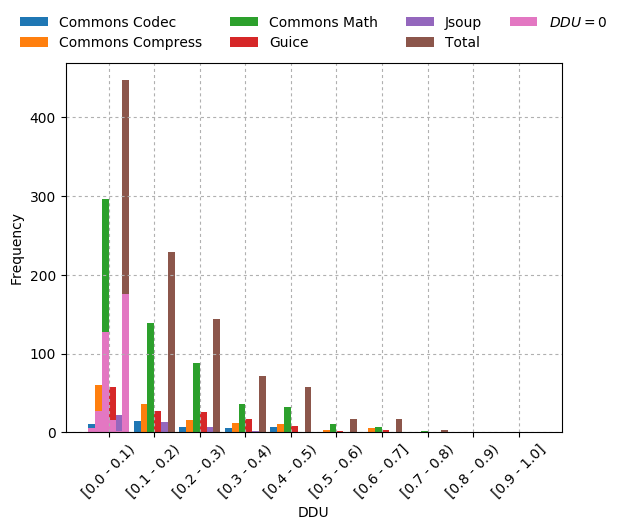
\includegraphics[width=\linewidth]{figures/grouped_barchart_ddu}
    \caption{DDU distribution.}%
    \label{fig:ddu}
\end{figure}

\begin{table}[]
\scriptsize
\centering
\caption{Activity matrix of \texttt{org.apache.commons.math4.analysis.function.Min}, \(\rho' = 1.0 \), \(\mathcal{G} = 0.809 \), \(\mathcal{U} = 1.0 \), and \(DDU = 0.809\).}%
\label{tab:min}
\begin{tabular}{l|cccc}
transaction & \(c_1 \) & \(c_2 \) & \(c_3 \) & \(c_4 \) \\ \hline
\texttt{UnivariateDifferentiableFunctionTest\#testMinus} & 1 & 0 & 1 & 1 \\
\texttt{FunctionUtilsTest\#testCollector} & 0 & 1 & 0 & 0 \\
\texttt{FunctionUtilsTest\#testAdd} & 1 & 0 & 1 & 0 \\
\texttt{FunctionUtilsTest\#testComposeDifferentiable} & 0 & 0 & 1 & 1 \\
\texttt{FunctionUtilsTest\#testCombine} & 1 & 0 & 1 & 0 \\
\texttt{FunctionUtilsTest\#testCompose} & 1 & 0 & 1 & 0 \\
\texttt{FunctionUtilsTest\#testAddDifferentiable} & 0 & 0 & 1 & 1
\end{tabular}
\end{table}

In \Cref{tab:min}, we observe a class with a high DDU\@: 0.809.
Its DDU is high because it has an optimal normalized density, uniqueness, and an almost optimal diversity.

\begin{table}[]
\scriptsize
\centering
\caption{Partial activity matrix of \texttt{org.jsoup.parser.ParseSettings}, \(\rho' = 0.727 \), \(\mathcal{G} = 0.204 \), \(\mathcal{U} = 0.555 \), and \(DDU = 0.082\).}%
\label{tab:parsesettings}
\begin{tabular}{l|ccccccccc}
transaction & \(c_1 \) & \(c_2 \) & \(c_3 \) & \(c_4 \) & \(c_5 \) & \(c_6 \) & \(c_7 \) & \(c_8 \) & \(c_9 \) \\ \hline
\texttt{ParseTest\#testBaidu} & 0 & 1 & 1 & 0 & 0 & 1 & 1 & 1 & 1 \\
\texttt{AttributesTest\#html} & 0 & 0 & 1 & 0 & 0 & 0 & 1 & 1 & 0 \\
\texttt{HtmlParserTest\#canPreserveAttributeCase} & 0 & 1 & 1 & 0 & 0 & 0 & 1 & 1 & 1 \\
\texttt{HtmlParserTest\#handlesBaseTags} & 0 & 1 & 1 & 0 & 0 & 1 & 1 & 1 & 1 \\
\texttt{SelectorTest\#descendant} & 0 & 1 & 1 & 0 & 0 & 1 & 1 & 1 & 1 \\
\vdots & \vdots & \vdots & \vdots & \vdots & \vdots & \vdots & \vdots & \vdots & \vdots
\end{tabular}
\end{table}

In \Cref{tab:parsesettings}, we observe a class with a low DDU\@: 0.082.
Eventhough the normalized density and uniqueness are above average, the DDU is low due to the low diversity.

\section{Observations}
In this section, we summarize our findings with regards to normalized density, diversity, uniqueness, and DDU\@.

The optimal normalized density is 1.0 and the optimal density is 0.5 for a test suite.
It is difficult to utilize normalized density to recommend the developer what kind of test to write --- a test that covers a few components or a test that covers many components.
For example, if \(\rho' = 0.6 \), then the density can either be \(\rho = 0.3 \) or \(\rho = 0.7 \).
Therefore, the density can be used to guide the developer in writing tests.
For example, when the test suite's density is less than 0.5, it is recommended to write tests that cover many components.
Conversely, when the test suite's density is greater than 0.5, it is recommended to write tests that cover a few components.

% In \Cref{tab:providesmethodscanner}, we observed that the more components a class has, the greater the impact of a test, that covers a relative small number of components, has on the sparseness of the activity matrix.
% Therefore, we pose the question whether density should be this punishing

In practice, we write tests to account for many corner cases.
From the diagnostic perspective, adding tests, that do not improve the information gain, is useless.
For example, the diversity can be negatively impacted when we write parameterized tests with certain inputs that cause identical activation patterns.
Another example is property-based testing, where the outputs are checked against a so-called \emph{property} that should hold true given arbitrary inputs that meet certain criteria.
Therefore, we pose the question whether we need a metric that penalizes tests that have identical component coverage.

% For DDU the density is normalized such that its operating domain is [0, 1].
% However, due to the definition of uniqueness, see \Cref{eq:uniqueness}, its domain is actually (0, 1] instead of [0, 1].

We observe in \Cref{fig:ddu}, that the DDU distribution is right-tailed.
This can be explained by the fact that the DDU is the product of normalized density, diversity, and uniqueness, which all operate in the domain [0, 1].
Even when a test suite has a high normalized density and diversity but a low uniqueness, then the value for DDU can only be as high as the uniqueness.
In other words, the DDU can only be as high as the term with the lowest value.
A possible solution to the right-tailed distribution is to use geometric mean.

% Multiplying the individual terms might not be the right approach.
%
% Based on the uniqueness observations, it seems that uniqueness at least requires the developer to write tests that cover a few components.

Revisiting the first research question:
\begin{framed}
\noindent
\textbf{RQ1:} How do normalized density, diversity, uniqueness, and DDU vary in practice?
\end{framed}
\textbf{A:} We observed that the average for normalized density, diversity, and uniqueness are 0.5145, 0.588, 0.477, respectively.
However, the values for DDU have an average of 0.157.
In addition, the distribution of DDU is right-tailed which could be explained by the fact that DDU can only be as high as the lowest component --- normalized density, diversity, or uniqueness.


\chapter{DDU vs. Diagnosability}%
\label{ch:rq2}
\begin{framed}
\noindent
\textbf{RQ2:} What is the relation between density, diversity, uniqueness, and DDU and diagnosability?
\end{framed}
In prior work, Perez \etal~\cite{DBLP:conf/icse/PerezAD17} show that optimizing test suite generation with respect to DDU results in better fault diagnosis.
Optimizing test suite generation with respect to DDU yields a 34\% increase in diagnostic performance compared to a test suite optimized for branch coverage.
Therefore, in this chapter, we perform experiments to verify the correlation between DDU and diagnosability.

\section{Experimental Setup}%
\label{sec:rq2_experimental_setup}
To verify the correlation between DDU and diagnosability, we seed 10 artificial multiple components faults of cardinality 2 --- that is, faults that are caused by two components --- for each class that has at least 8 components, i.e.\ branches.
We do not seed single component faults because in this case the optimal activity matrix for diagnosability is an identity matrix, i.e.\ each component is tested individually by a (very focused unit) test.

For each injected fault, we produce an error vector corresponding to the activity matrix and the fault.
We determine for each test that exercises the faulty components whether it is failing according to an \emph{oracle quality probability} of 0.75, which was also used in prior work~\cite{DBLP:conf/icse/PerezAD17}.
Note that we only seed faults that result in at least one failing test in the error vector because in this experiment we are interested in diagnosability and not error detection.
For some classes, it is not possible to seed 10 faults that result in a failing test in the error vector and, therefore, we do not include these classes in the experiment.

Then, for each seeded program spectrum, we use \textsc{Staccato} to generate fault candidates and \textsc{Barinel} to rank these candidates into a diagnostic report, see \Cref{sec:sbr} for a more detailed explanation.
Based on the diagnostic report we compute the wasted effort which is a measurement for diagnosability.
This whole process of constructing an activity matrix, injecting artificial faults, performing SFL, and diagnosis evaluation is shown in \Cref{fig:fault_generation}.

To account for randomness of generating fault sets, we repeat this process 10 times.
Additionally, \textsc{Staccato} can sometimes take hours or days to generate fault candidates.
Hence, we discard classes when the generation of fault candidates takes longer than 10 seconds; this resulted in 15 classes being discarded.
In \Cref{tab:too_big}, we observe that the discarded classes are covered by a relative big number of tests and consist of many branches, potentially causing \textsc{Staccato}'s computation to take longer than 10 seconds.

\begin{table}[]
    \centering
    \caption{Classes that were not included in the analysis due to \textsc{Staccato} taking longer than 10 seconds.}%
    \label{tab:too_big}
    \begin{adjustbox}{center}
    \begin{tabular}{lrr}
        \toprule
        Class & Number of tests & Number of branches \\ \rowcolor{Gray}
        com.google.inject.AbstractModule & 643 & 27 \\ 
        com.google.inject.internal.InjectorImpl & 601 & 223 \\ \rowcolor{Gray}
        com.google.inject.spi.Elements & 706 & 109 \\ 
        org.apache.commons.math4.analysis.differentiation.DSCompiler & 278 & 338 \\ \rowcolor{Gray}
        org.apache.commons.math4.linear.AbstractFieldMatrix & 140 & 295 \\ 
        org.apache.commons.math4.linear.AbstractRealMatrix & 559 & 262 \\ \rowcolor{Gray}
        org.apache.commons.math4.linear.BlockRealMatrix & 221 & 374 \\ 
        org.apache.commons.math4.linear.QRDecomposition & 108 & 101 \\ \rowcolor{Gray}
        org.apache.commons.math4.util.Decimal64 & 222 & 147 \\ 
        org.apache.commons.math4.util.FastMath & 3646 & 702 \\ \rowcolor{Gray}
        org.apache.commons.math4.util.MathArrays & 1261 & 306 \\ 
        org.jsoup.nodes.Element & 426 & 233 \\ \rowcolor{Gray}
        org.jsoup.parser.HtmlTreeBuilder & 406 & 941 \\ 
        org.jsoup.parser.HtmlTreeBuilderState & 392 & 673 \\ \rowcolor{Gray}
        org.jsoup.parser.TokeniserState & 406 & 439 \\
        \bottomrule
    \end{tabular}
    \end{adjustbox}
\end{table}

\begin{figure}
  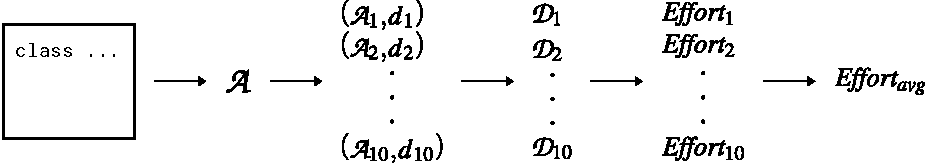
\includegraphics[width=\linewidth]{figures/effort_approach}
  \caption{An activity matrix \(\mathcal{A} \) is constructed from a particular class. Then, 10 fault candidates of cardinality 2 are seeded with a corresponding activity matrix \(\mathcal{A}_k \). For each seeded matrix, we perform fault diagnosis with \textsc{Barinel} resulting in diagnostic report \(\mathcal{D}_k \) and compute the wasted effort. Finally, we compute the average wasted effort. This process is repeated 10 times.}%
  \label{fig:fault_generation}
\end{figure}

\begin{figure}
  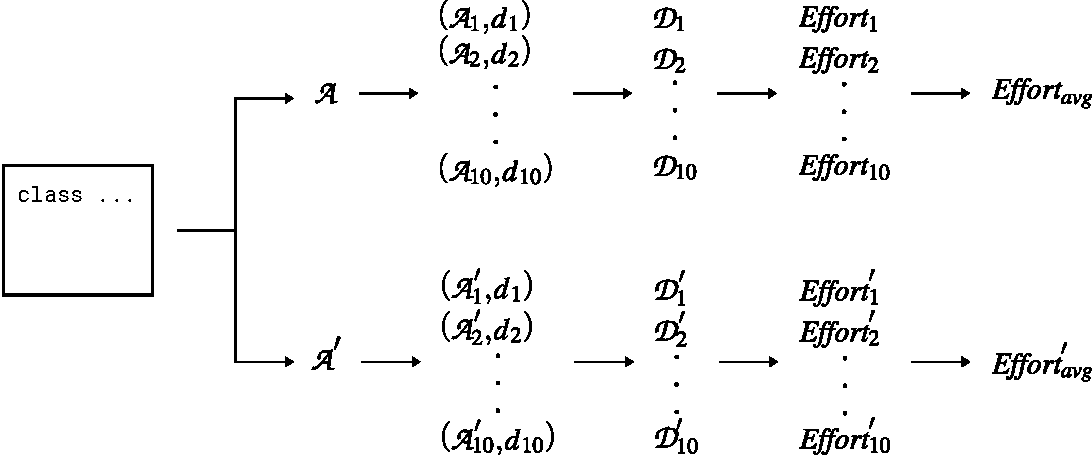
\includegraphics[width=\linewidth]{figures/delta_effort_approach}
  \caption{Two activity matrices \(\mathcal{A} \) and \(\mathcal{A}' \) are produced for a particular class based on two different test suites. We seed 10 fault candidates of cardinality 2 and accordingly produce 10 activity matrices. Then, we use \textsc{Barinel} to perform fault diagnosis and compute the wasted effort.}%
  \label{fig:fault_generation_delta}
\end{figure}

In the construction of the activity matrix we use the branch granularity, that is, every column in the activity matrix represents a method branch.
This granularity is also used by Perez \etal~\cite{DBLP:conf/icse/PerezAD17}.
To construct the activity matrix of a class we use Perez' DDU Maven plugin\footnote{\url{https://github.com/aperez/ddu-maven-plugin}} using the \texttt{basicblock} granularity, which represents branch granularity.
The steps after obtaining the activity matrix in \Cref{fig:fault_generation} are performed using Python scripts\footnote{\url{https://github.com/aaronang/ddu}}.

This experiment is different from Perez \etal's work because we do not improve the DDU of a fixed system.
In Perez \etal's study, the authors improved the DDU of a fixed system under test by generating tests using \emph{EvoSuite}.
However, in this experiment, we compute the DDU for each class and measure for each class its diagnosability using the aforementioned approach.

For this reason, we perform another experiment where we generate two test suites for each class with at least 8 components and at least 10 tests.
We generate two test suites by enabling the first 50\% of the tests and 100\% of the tests.
For both test suites we compute the DDU and randomly seed 10 multiple components faults of cardinality 2 to compute the wasted effort.
Similar to previous experiment we perform this process 10 times to account for randomness of generating fault sets.
The intuition behind this experiment is when we improve the DDU of a fixed system, its diagnosability should improve too.
If the two created test suites of a class do result in a difference in DDU, then the class is discarded.
The setup of this experiment is illustrated in \Cref{fig:fault_generation_delta}.

In the experiments, we compute the wasted effort using the following approach.
Given a diagnostic report where the candidates are ranked by their fault probabilities in descending order, shown in \Cref{tab:diagnostic_report}, and the injected fault set: \(\langle c_0, c_1 \rangle \), the wasted effort is computed by, first, flattening the ranked list to single components and recomputing the probabilities for each component using addition, e.g.\ fault probability of \(\langle c_0 \rangle = 0.5 + 0.05 = 0.55\).
Then, the wasted effort is computed for each component in the generated fault set: \(\emph{effort}_{c_0} = \frac{0}{4} = 0\), \(\emph{effort}_{c_1} = \frac{1}{4} = 0.25\).
Finally, the wasted effort of the seeded multi-component fault is computed by averaging the computed wasted efforts: \(\frac{0 + 0.25}{2} = 0.125\).
This approach is used because of its simplicity.
It's not always guaranteed that the multi-component fault is found as a candidate in the diagnostic report.
For example, there are cases that \textsc{Staccato} does not generate \(c_0\) and \(c_1\) as one candidate set but as separate candidates.
\begin{table}[]
    \centering
    \scriptsize
    \caption{Computation of wasted effort.}%
    \label{tab:diagnostic_report}
    \begin{subtable}{.5\linewidth}
      \centering
        \caption{Diagnostic report computed by \textsc{Barinel}.}
        \begin{tabular}{l|l}
            candidate & fault probability \\ \hline
            \(\langle c_0, c_1 \rangle \) & 0.5 \\
            \(\langle c_2 \rangle \) & 0.3 \\
            \(\langle c_3 \rangle \) & 0.15 \\
            \(\langle c_0 \rangle \) & 0.05 \\
        \end{tabular}
    \end{subtable}%
    \begin{subtable}{.5\linewidth}
      \centering
        \caption{Flatten candidates and rerank.}
        \begin{tabular}{l|l}
            candidate & fault probability \\ \hline
            \( c_0 \) & 0.55 \\
            \(c_1 \) & 0.5 \\
            \(c_2 \) & 0.3 \\
            \(c_3 \) & 0.15 \\
        \end{tabular}
    \end{subtable}
\end{table}

\section{Experimental Results}%
\label{sec:rq2_experimental_results}

\begin{figure*}
    \centering
    \begin{subfigure}[t]{0.49\linewidth}
        \centering
        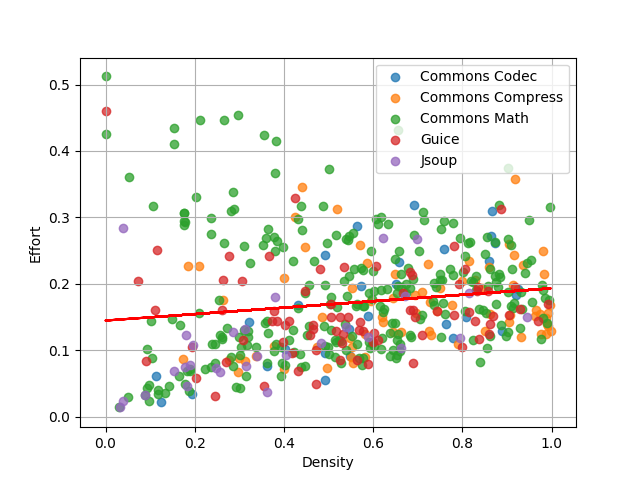
\includegraphics[width=\linewidth]{figures/effort_density}
        \caption{Normalized density, \(r = 0.183 \), \(p < 0.001 \).}%
        \label{fig:effort_density}
    \end{subfigure}
    \hfill
    \begin{subfigure}[t]{0.49\linewidth}
        \centering
        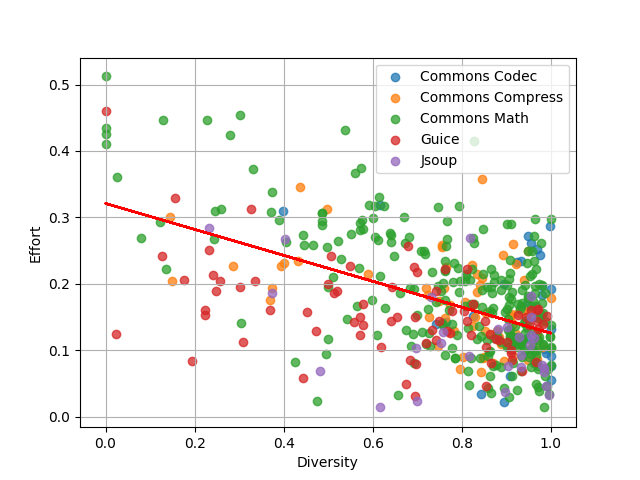
\includegraphics[width=\linewidth]{figures/effort_diversity}
        \caption{Diversity, \(r = -0.326 \), \(p < 0.001 \).}%
        \label{fig:effort_diversity}
    \end{subfigure}
    \vskip\baselineskip%
    \begin{subfigure}[b]{0.49\linewidth}
        \centering
        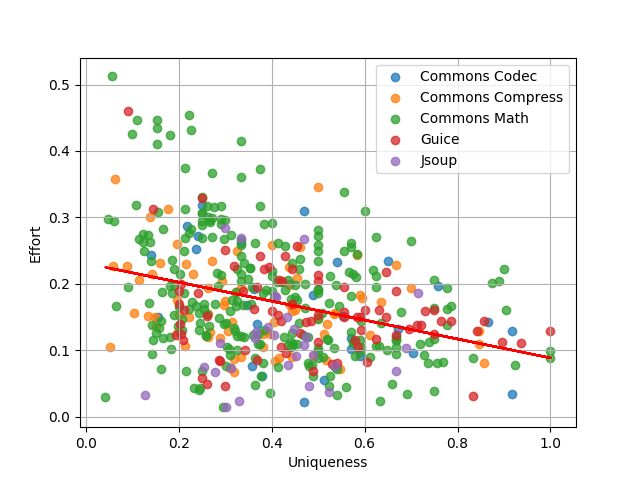
\includegraphics[width=\linewidth]{figures/effort_uniqueness}
        \caption{Uniqueness, \(r = -0.120 \), \(p < 0.001 \).}%
        \label{fig:effort_uniqueness}
    \end{subfigure}
    \hfill
    \begin{subfigure}[b]{0.49\linewidth}
        \centering
        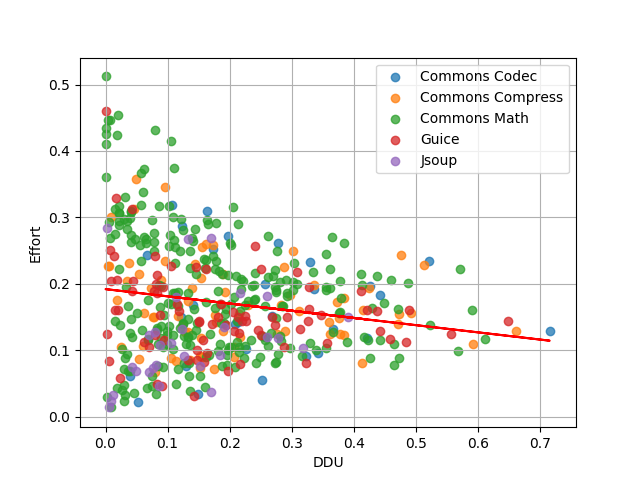
\includegraphics[width=\linewidth]{figures/effort_ddu}
        \caption{DDU, \(r = -0.046 \), \(p = 0.224 \).}%
        \label{fig:effort_ddu}
    \end{subfigure}
    \caption{Scatterplot of density, diversity, uniqueness, and DDU against effort.}%
    \label{fig:metric_vs_effort}
\end{figure*}

In the first experiment, we measure for each class the normalized density, diversity, uniqueness, DDU, and effort.
The results of this experiment are shown in \Cref{fig:metric_vs_effort}.
In \Cref{fig:metric_vs_effort}, the population comprises all classes of all projects.
Each datapoint in \Cref{fig:metric_vs_effort} represents a class for which 100 fault candidates are generated in (potentially overlapping) sets of 10 fault candidates as described in \Cref{fig:fault_generation}.

Using a significance level of 5\%, we observe the that there is a weak positive correlation between density and effort, a weak negative correlation between diversity and effort, a weak negative correlation between uniqueness and effort, and a statistically non-significant weak correlation between DDU and effort.

To investigate the relations between these metrics in more detail, we display the correlation values \emph{per project} in \Cref{tab:correlation_effort}.
For three projects we can say with 95\% confidence that normalized density is correlated with effort.
However, the Pearson correlation for Commons Compress is negative while the Pearson correlation values for Commons Math and Commons Codec are positive.
Hence, the results show no strong evidence that density is strongly correlated with effort.

Regarding diversity and uniqueness, we observe in \Cref{tab:correlation_effort} and \Cref{fig:metric_vs_effort} that both metrics have a weak negative correlation with effort, and that the correlation values in 4 out of 5 projects are statistically significant.

Regarding DDU, for two projects the results show statistical significance that DDU has a weak negative correlation with effort.
However, for three projects there is no evidence that DDU is correlated to effort.
Therefore, there is no strong evidence that DDU is negatively correlated to effort.

\begin{table}[]
\centering
\caption{Correlations between density, diversity, uniqueness, DDU, and effort for each project.}%
\label{tab:correlation_effort}
\begin{adjustbox}{center}
\begin{tabular}{llllll}
\toprule
 &  & \multicolumn{4}{c}{Pearson correlation / Correlation p-value} \\ \cline{3-6}
\multirow{-2}{*}{Subject} & \multirow{-2}{2cm}{Number of classes} & Density & Diversity & Uniqueness & DDU \\
\rowcolor{Gray}
\cellcolor{Gray} & \cellcolor{Gray} & \textbf{0.63} & -0.33 & \textbf{-0.65} & -0.23 \\
\rowcolor{Gray}
\multirow{-2}{*}{\cellcolor{Gray}\begin{tabular}[c]{@{}l@{}}Commons\\ Codec\end{tabular}} & \multirow{-2}{*}{\cellcolor{Gray}34} & \(5.880\times10^{-5} \) & 0.057 & \(3.713\times10^{-5} \) & 0.197 \\
 &  & \textbf{-0.22} & \textbf{-0.45} & \textbf{-0.40} & \textbf{-0.37} \\
\multirow{-2}{*}{\begin{tabular}[c]{@{}l@{}}Commons\\ Compress\end{tabular}} & \multirow{-2}{*}{104} & \(0.027 \) & \(1.348\times10^{-6} \) & \(2.083\times10^{-5} \) & \(1.121\times10^{-4} \) \\
\rowcolor{Gray}
\cellcolor{Gray} & \cellcolor{Gray} & \textbf{0.20} & \textbf{-0.36} & \textbf{-0.19} & -0.03 \\
\rowcolor{Gray}
\multirow{-2}{*}{\cellcolor{Gray}\begin{tabular}[c]{@{}l@{}}Commons\\ Math\end{tabular}} & \multirow{-2}{*}{\cellcolor{Gray}420} & \(4.982\times10^{-5} \) & \(1.782\times10^{-14} \) & \(7.553\times10^{-5} \) & 0.572 \\
 &  & 0.01 & \textbf{-0.31} & \textbf{-0.29} & \textbf{-0.22} \\
\multirow{-2}{*}{Guice} & \multirow{-2}{*}{94} & 0.935 & \(0.002 \) & \(0.005 \) & \(0.031 \) \\
\rowcolor{Gray}
\cellcolor{Gray} & \cellcolor{Gray} & 0.29 & \textbf{-0.37} & 0.16 & 0.20 \\
\rowcolor{Gray}
\multirow{-2}{*}{\cellcolor{Gray}Jsoup} & \multirow{-2}{*}{\cellcolor{Gray}37} & 0.085 & \(0.024 \) & 0.337 & 0.229\\
\bottomrule
\end{tabular}
\end{adjustbox}
\end{table}

\begin{table}[]
    \scriptsize
    \centering
    \caption{Partial activity matrix of \texttt{com.google.inject.internal.AbstractProcessor}, \(\rho = 1 \), \(\rho' = 0 \).}%
    \label{tab:abstractprocessor}
    \begin{adjustbox}{center}
    \begin{tabular}{l|ccccccccccc}
    transaction & \(c_1 \) & \(c_2 \) & \(c_3 \) & \(c_4 \) & \(c_5 \) & \(c_6 \) & \(c_7 \) & \(c_8 \) & \(c_9 \) & \(c_{10} \) & \(c_{11} \) \\ \hline
    \texttt{com.google.inject.BinderTest\#testUntargettedBinding} & 1 & 1 & 1 & 1 & 1 & 1 & 1 & 1 & 1 & 1 & 1 \\
    \texttt{com.google.inject.BinderTest\#testMissingDependency} & 1 & 1 & 1 & 1 & 1 & 1 & 1 & 1 & 1 & 1 & 1 \\
    \texttt{com.google.inject.BinderTest\#testProviderFromBinder} & 1 & 1 & 1 & 1 & 1 & 1 & 1 & 1 & 1 & 1 & 1 \\
    \vdots & \vdots & \vdots & \vdots & \vdots & \vdots & \vdots & \vdots & \vdots & \vdots & \vdots & \vdots \\
    \texttt{com.googlecode.guice.Jsr330Test\#testInjecting\dots} & 1 & 1 & 1 & 1 & 1 & 1 & 1 & 1 & 1 & 1 & 1 \\
    \texttt{com.googlecode.guice.Jsr330Test\#testScopeAnnotation} & 1 & 1 & 1 & 1 & 1 & 1 & 1 & 1 & 1 & 1 & 1 \\
    \texttt{com.googlecode.guice.Jsr330Test\#testInject} & 1 & 1 & 1 & 1 & 1 & 1 & 1 & 1 & 1 & 1 & 1 \\
    \end{tabular}
    \end{adjustbox}
\end{table}

It is unexpected that the normalized density tends to be positively correlated to wasted effort.
The normalized density is a diagnosability assessment metric and is supposed to be negatively correlated to wasted effort, that is, the higher the normalized density, the better the diagnosability and, thus, the lower the wasted effort.
In \Cref{fig:effort_density}, the three datapoints in the top-left corner (\(\rho' = 0 \wedge \emph{effort} > 0.4\)) are classes --- \texttt{Abstract\-Processor}, \texttt{Iterative\-Legendre\-Gauss\-Integrator}, \texttt{Circle\-Vectorial} --- that have an activity matrix where \(\rho = 1\) resulting in a normalized density \(\rho' = 0\).
In \Cref{tab:abstractprocessor}, the partial activity matrix of \texttt{AbstractProcessor} is shown.
During the candidate generation phase using \textsc{Staccato}, the following fault candidates are generated: \(\langle c_1 \rangle \), \(\langle c_2 \rangle \), \(\langle c_3 \rangle \), \(\langle c_4 \rangle \), \(\langle c_5 \rangle \), \(\langle c_6 \rangle \), \(\langle c_7 \rangle \), \(\langle c_8 \rangle \), \(\langle c_9 \rangle \), \(\langle c_{10} \rangle \), \(\langle c_{11} \rangle \).
\textsc{Barinel} will rank these candidates randomly because each component is involved in all transactions.
Hence, the diagnostic performance of these three classes is as good as randomly investingating components and, thus, the wasted effort for these classes is around 0.5.

The datapoints in the bottom-left corner (\(\rho' < 0.1 \wedge \emph{effort} < 0.05\)), in \Cref{fig:effort_density} are classes that have a low density.
Since we are only including classes for which we can generate 10 faults that result in a failing test in the error vector, these classes have a high diagnosability for the generated faults and, thus, a low wasted effort.

In the top-right corner of \Cref{fig:effort_density} (\(\rho' > 0.8 \wedge \emph{effort} > 0.3 \)), the classes have a higher wasted effort than the classes in the bottom-right corner (\(\rho' > 0.8 \wedge \emph{effort} < 0.15 \)) because the activity matrices consist mostly of tests that cover many components.
For example, in \Cref{tab:dormandprince}, we observe that most transactions cover all components making it difficult for SBR to diagnose the faults accurately.
In \Cref{tab:baseoptimizer}, we observe the class \texttt{BaseOptimizer}'s activity matrix which mostly consists of tests that cover a few components, enabling SBR to diagnose faults better.
Note that there are classes in the top-right corner of \Cref{fig:effort_density} for which the activity matrix looks similar to \Cref{tab:baseoptimizer} and, therefore, it is unclear what exactly causes the diagnosability to be good or bad for classes where \(\rho' > 0.8\).
 
\begin{table}[]
    \scriptsize
    \centering
    \caption{Partial activity matrix of \texttt{org.\-apache.\-commons.\-math4.\-ode.\-nonstiff.\-Dormand\-Prince853\-Field\-Step\-Interpolator}, \(\rho' = 902 \).}%
    \label{tab:dormandprince}
    \begin{adjustbox}{center}
    \begin{tabular}{l|ccccccccccccccc}
    transaction & \(c_1 \) & \(c_2 \) & \(c_3 \) & \(c_4 \) & \(c_5 \) & \(c_6 \) & \(c_7 \) & \(c_8 \) & \(c_9 \) & \(c_{10} \) & \(c_{11} \) & \(c_{12} \) & \(c_{13} \) & \(c_{14} \) \\ \hline
    \texttt{testModelsMerging} & 1 & 1 & 1 & 0 & 1 & 1 & 1 & 1 & 0 & 1 & 1 & 1 & 1 & 1 \\
    \texttt{testStartFailure} & 0 & 0 & 0 & 0 & 0 & 0 & 1 & 0 & 0 & 0 & 0 & 0 & 0 & 0 \\
    \texttt{testEvents} & 1 & 1 & 1 & 1 & 1 & 1 & 1 & 1 & 1 & 1 & 1 & 1 & 1 & 1 \\
    \end{tabular}
    \end{adjustbox}
\end{table}

\begin{table}[]
    \scriptsize
    \centering
    \caption{Partial activity matrix of \texttt{org.\-apache.\-commons.\-math4.\-optim.\-Base\-Optimizer}, \(\rho' = 0.976 \).}%
    \label{tab:baseoptimizer}
    \begin{adjustbox}{center}
    \begin{tabular}{l|cccccccccccccccc}
    transaction & \(c_1 \) & \(c_2 \) & \(c_3 \) & \(c_4 \) & \(c_5 \) & \(c_6 \) & \(c_7 \) & \(c_8 \) & \(c_9 \) & \(c_{10} \) & \(c_{11} \) & \(c_{12} \) & \(c_{13} \) & \(c_{14} \) & \(c_{15} \) & \(c_{16} \) \\ \hline
    \texttt{testDimensionMatch} & 0 & 0 & 0 & 0 & 1 & 0 & 0 & 0 & 0 & 1 & 1 & 0 & 0 & 0 & 0 & 1 \\
    \texttt{testBoundariesDimensionMismatch} & 0 & 0 & 0 & 0 & 1 & 0 & 0 & 0 & 0 & 1 & 1 & 0 & 0 & 1 & 0 & 1 \\
    \texttt{testMissingMaxEval} & 0 & 0 & 0 & 0 & 1 & 0 & 0 & 0 & 0 & 1 & 1 & 0 & 1 & 0 & 0 & 1 \\
    \texttt{testMissingSearchInterval} & 0 & 0 & 0 & 0 & 1 & 0 & 0 & 0 & 0 & 1 & 1 & 0 & 1 & 1 & 0 & 1 \\
    \texttt{testMath290GEQ} & 0 & 0 & 0 & 0 & 1 & 0 & 0 & 0 & 0 & 1 & 1 & 1 & 0 & 0 & 0 & 1 \\
    \texttt{testAckley} & 0 & 0 & 1 & 0 & 1 & 0 & 1 & 0 & 0 & 1 & 1 & 0 & 0 & 1 & 0 & 1 \\
    \texttt{testBadFunction} & 0 & 0 & 1 & 0 & 1 & 0 & 1 & 0 & 1 & 1 & 1 & 0 & 1 & 1 & 0 & 1 \\
    \texttt{testMaxEvaluations} & 0 & 0 & 1 & 1 & 1 & 0 & 1 & 0 & 0 & 1 & 1 & 0 & 0 & 1 & 0 & 1 \\
    \texttt{testMath842Cycle} & 1 & 0 & 0 & 0 & 1 & 0 & 0 & 0 & 0 & 1 & 1 & 0 & 0 & 0 & 0 & 1 \\
    \texttt{testDegeneracy} & 1 & 0 & 0 & 0 & 1 & 0 & 0 & 0 & 0 & 1 & 1 & 1 & 0 & 0 & 0 & 1 \\
    \texttt{testSolutionCallback} & 1 & 0 & 0 & 0 & 1 & 0 & 0 & 1 & 0 & 1 & 1 & 1 & 0 & 0 & 0 & 1 \\
    \texttt{testBoundaries} & 1 & 0 & 0 & 0 & 1 & 0 & 1 & 0 & 0 & 1 & 1 & 0 & 1 & 1 & 0 & 1 \\
    \texttt{testAckley} & 1 & 0 & 0 & 0 & 1 & 1 & 1 & 0 & 0 & 1 & 1 & 0 & 1 & 1 & 0 & 1 \\
    \texttt{testQuinticMax} & 1 & 0 & 0 & 1 & 1 & 0 & 1 & 0 & 0 & 1 & 1 & 0 & 1 & 1 & 0 & 1 \\
    \texttt{testMaxIterations} & 1 & 0 & 0 & 1 & 1 & 1 & 1 & 0 & 0 & 1 & 1 & 0 & 1 & 1 & 0 & 1 \\
    \texttt{testQuinticMin} & 1 & 0 & 1 & 0 & 1 & 0 & 1 & 0 & 0 & 1 & 1 & 0 & 1 & 1 & 0 & 1 \\
    \texttt{testQuinticMin} & 1 & 0 & 1 & 0 & 1 & 0 & 1 & 0 & 1 & 1 & 1 & 0 & 1 & 1 & 0 & 1 \\
    \texttt{testLeastSquares1} & 1 & 0 & 1 & 0 & 1 & 1 & 1 & 0 & 0 & 1 & 1 & 0 & 1 & 1 & 0 & 1 \\
    \texttt{testCircleFitting} & 1 & 0 & 1 & 0 & 1 & 1 & 1 & 0 & 1 & 1 & 1 & 0 & 1 & 1 & 0 & 1 \\
    \texttt{testSinMin} & 1 & 0 & 1 & 1 & 1 & 0 & 1 & 0 & 1 & 1 & 1 & 0 & 1 & 1 & 0 & 1 \\
    \end{tabular}
    \end{adjustbox}
\end{table}

\begin{figure*}
    \centering
    \begin{subfigure}[b]{0.49\linewidth}
        \centering
        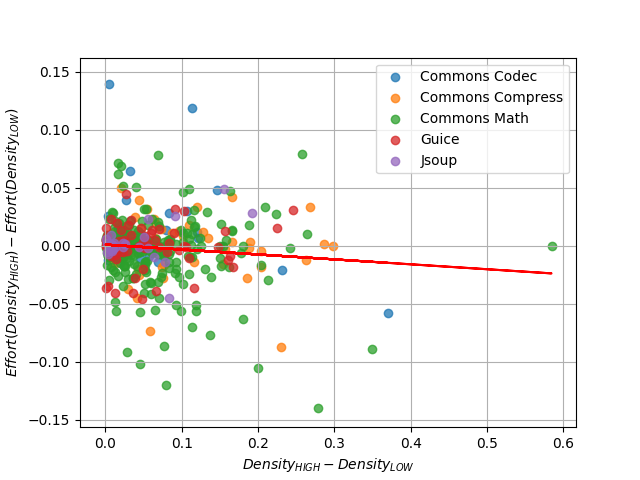
\includegraphics[width=\linewidth]{figures/delta_effort_density}
        \caption{Density, \(r=-0.107 \), \(p<0.01 \).}%
        \label{fig:delta_effort_density}
    \end{subfigure}
    \hfill
    \begin{subfigure}[b]{0.49\linewidth}
        \centering
        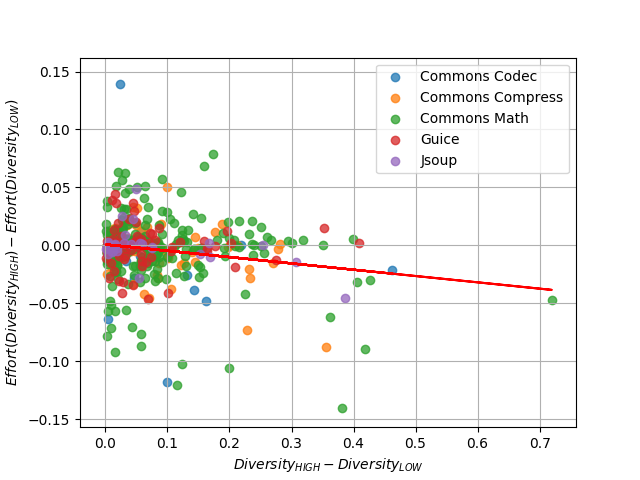
\includegraphics[width=\linewidth]{figures/delta_effort_diversity}
        \caption{Diversity, \(r=-0.189 \), \(p = 4.479\times10^{-5} \).}%
        \label{fig:delta_effort_diversity}
    \end{subfigure}
    \vskip\baselineskip%
    \begin{subfigure}[b]{0.49\linewidth}
        \centering
        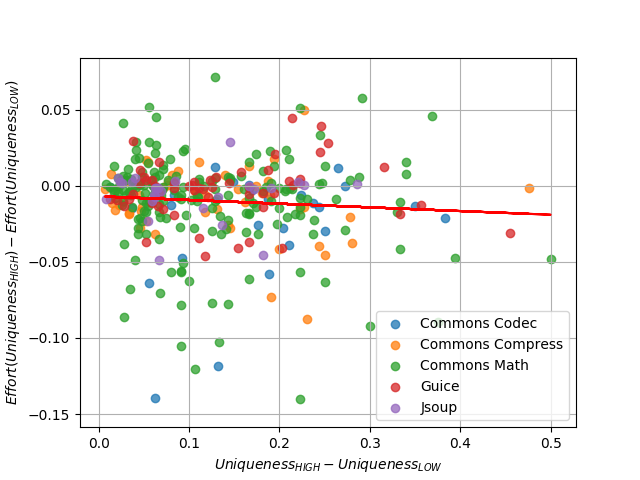
\includegraphics[width=\linewidth]{figures/delta_effort_uniqueness}
        \caption{Uniqueness, \(r=-0.079 \), \(p=0.137 \).}%
        \label{fig:delta_effort_uniqueness}
    \end{subfigure}
    \hfill
    \begin{subfigure}[b]{0.49\linewidth}
        \centering
        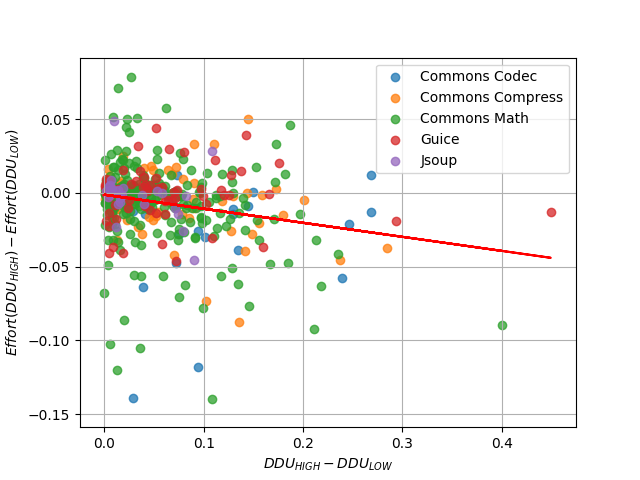
\includegraphics[width=\linewidth]{figures/delta_effort_ddu}
        \caption{DDU, \(r=-0.223 \), \(p=9.044\times10^{-7} \).}%
        \label{fig:delta_effort_ddu}
    \end{subfigure}
    \caption{Scatterplot of delta density, delta diversity, delta uniqueness, and delta DDU against delta effort.}%
    \label{fig:delta_metric_vs_delta_effort}
\end{figure*}

\begin{table}[]
\centering
\caption{Correlations between delta normalized density, delta diversity, delta uniqueness, delta DDU, and delta effort for each project.}%
\label{tab:delta_metric_delta_effort}
\begin{adjustbox}{center}
\begin{tabular}{lllll}
\toprule
 & \multicolumn{4}{c}{Size / Pearson correlation / Correlation p-value} \\
\multirow{-2}{*}{Subject} & Density & Diversity & Uniqueness & DDU \\
\rowcolor{Gray}
\cellcolor{Gray} & 29 & 24 & 26 & 29 \\
\rowcolor{Gray}
\cellcolor{Gray} & -0.277 & -0.229 & 0.230 & 0.011 \\
\rowcolor{Gray}
\multirow{-3}{*}{\cellcolor{Gray}\begin{tabular}[c]{@{}l@{}}Commons\\ Codec\end{tabular}} & 0.145 & 0.281 & 0.256 & 0.950 \\
 & 74 & 73 & 55 & 74 \\
 & -0.098 & \textbf{-0.372} & -0.217 & \textbf{-0.297} \\
\multirow{-3}{*}{\begin{tabular}[c]{@{}l@{}}Commons\\ Compress\end{tabular}} & 0.401 & \(0.001 \) & 0.111 & \(0.010 \) \\
\rowcolor{Gray}
\cellcolor{Gray} & 251 & 256 & 186 & 262 \\
\rowcolor{Gray}
\cellcolor{Gray} & \textbf{-0.142} & \textbf{-0.162} & -0.109 & \textbf{-0.280} \\
\rowcolor{Gray}
\multirow{-3}{*}{\cellcolor{Gray}\begin{tabular}[c]{@{}l@{}}Commons\\ Math\end{tabular}} & \(0.023 \) & \(0.009 \) & 0.135 & \(3.855\times10^{-6} \) \\
 & 78 & 78 & 57 & 78 \\
 & 0.103 & 0.001 & 0.047 & -0.006 \\
\multirow{-3}{*}{Guice} & 0.368 & 0.995 & 0.728 & 0.952 \\
\rowcolor{Gray}
\cellcolor{Gray} & 29 & 29 & 27 & 29 \\
\rowcolor{Gray}
\cellcolor{Gray} & \textbf{0.452} & \textbf{-0.465} & 0.012 & -0.273 \\
\rowcolor{Gray}
\multirow{-3}{*}{\cellcolor{Gray}Jsoup} & \(0.013 \) & \(0.011 \) & 0.951 & 0.150\\
\bottomrule
\end{tabular}
\end{adjustbox}
\end{table}

In the second experiment, we generate two test suites for a given class: a test suite with the first 50\% of the test cases enabled, and a test suite with 100\% of the test cases enabled.
This naturally results in two test suites with two different DDU values.
For each class, we compare the effort of a test suite with a lower DDU value with a test suite with a higher DDU value.
Identical approach is used for normalized density, diversity, and uniqueness.
Note that we exclude classes where the two test suites do not result in a metric difference.
The results of this experiment are shown in \Cref{fig:delta_metric_vs_delta_effort} and \Cref{tab:delta_metric_delta_effort}.
In \Cref{fig:delta_metric_vs_delta_effort}, we observe that an increase in any metric --- normalized density, diversity, uniqueness, DDU --- results in a lower required effort to diagnose mistakes.
Although the results are statistically significant except for uniqueness, see \Cref{fig:delta_metric_vs_delta_effort}, the correlations are weak.

Revisiting the second research question:
\begin{framed}
\noindent
\textbf{RQ2:} What is the relation between density, diversity, uniqueness, and DDU and diagnosability?
\end{framed}
\textbf{A:} In the first experiment, we observe that diversity, uniqueness and DDU have a negative weak correlation with diagnosability.
The normalized density showed an unexpected weak positive correlation with diagnosability.
In the second experiment, we observe that an improvement in normalized density, diversity, uniqueness and DDU have a negative weak correlation with an improvement in diagnosability.
In conclusion, there is no strong evidence that indicates that the normalized density, diversity, uniqueness, DDU are strongly correlated with the diagnosability.
Consequently, this means that these diagnosability assessment metrics are, currently, only useful for generating test suites to improve diagnosability and SBFL techniques.

\chapter{DDU vs. Test Coverage}%
\label{ch:rq3}

\begin{framed}
\noindent
\textbf{RQ3:} What is the relation between density, diversity, uniqueness, and DDU and test coverage?
\end{framed}

In this chapter, we investigate the relation between DDU and test coverage.
The reason for researching the relation between DDU and test coverage is to investigate whether DDU should be used as a complementary metric to test coverage as Perez \etal\ proposed.
If there is a strong correlation between DDU and test coverage, then it means that DDU might function as an error detection metric too.
Furthermore, investigating the relation between DDU and test coverage might give us insight in how DDU and test coverage could work together in practice.

To answer the research question we will perform several experiments.
First, we confirm that test coverage is strongly correlated with error detection since test coverage presumably optimizes the test suite for error detection.
Second, we investigate the relation between DDU and test coverage.
Third, we examine the relation between DDU and error detection.


\section{Experimental Setup}
Similar to the previous experiment, we use the projects Commons Codec, Commons Compress, Commons Math, Guice, and Jsoup.

To analyze the relation between test coverage and error detection, we measure the test coverage and error detection.
Test coverage can be determined by dividing the number of components hit in the activity matrix by the total number of components in the activity matrix.
Given the acitity matrix in \Cref{tab:test_coverage}, we observe that 3 out of the 4 components are hit and therefore the test coverage is \(\frac{3}{4} = 0.75 \).
\begin{table}[]
\centering
\caption{Example of activity matrix with a test coverage of 75\%. Bolded components are hit by one of the tests.}%
\label{tab:test_coverage}
\begin{tabular}{l|llll}
transactions & \(\mathbf{c_1} \) & \(\mathbf{c_2} \) & \(c_3 \) & \(\mathbf{c_4} \) \\ \hline
\(t_1 \) & 0 & 0 & 0 & 1 \\
\(t_2 \) & 1 & 0 & 0 & 1 \\
\(t_3 \) & 1 & 1 & 0 & 0
\end{tabular}
\end{table}

The error detection is computed by generating 10 artificial faults --- in the experiments we generate multiple components faults with a cardinality 2.
As opposed to the experimental setup described in \Cref{sec:rq2_experimental_setup} where we only generate faults that cause a failure, in this experiment, we also include artificial faults that that do not cause a failure because we are interested in error detection.
For each fault, we compute the error vector using an \emph{oracle probability} of 0.75, similar to Perez \etal's study, and check whether the vector (\(e_i\)) contains an error, i.e. \( 1 \in e_i \).
Finally, the error detection \(\emph{ED}\) is computed by dividing the number of detected faults by 10, the number of generated faults.

To account for randomness of generating fault candidates, we repeat this process 10 times.
We obtain the activity matrices by using Perez \etal's \texttt{ddu-maven-plugin}, similar to the experiments in \Cref{ch:rq2}.
An overview of this experiment is illustrated in \Cref{fig:error_detection_computation}.
\begin{figure}[b]
  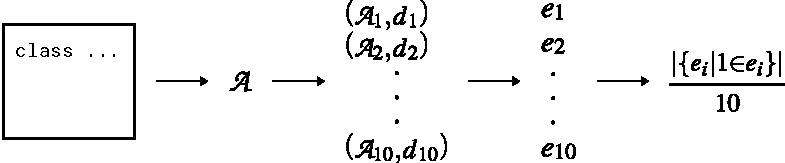
\includegraphics[width=\linewidth]{figures/error_detection}
  \caption{We compute the activity matrix for a given class and generate 10 artificial fault candidates \(d_1 \), \(d_2 \), \(d_{10}\) of cardinality 2. For each pair \((\mathcal{A}_i, d_i) \), the error vector \(e_i \) is computed. The error detection \(\emph{ED}\) is computed by dividing the number of detected faults by the number of generated faults.}%
  \label{fig:error_detection_computation}
\end{figure}

For the second experiment, in which we investigate the relation between DDU and test coverage, we compute the normalized density, diversity, uniqueness, DDU, and test coverage for each activity matrix, and compute the correlation.
Furthermore, we use a similar approach as the experiments in \Cref{ch:rq2}; we create two test suites: (1) a test suite that consists of the first 50\% of the available tests and (2) a test suite that consists of 100\% of the available tests.
This will most likely result in a system with two test suites with different DDU values, allowing us to investigate whether improving the DDU for a fixed system results in a test coverage improvement.
If the two created tests suites of class do not result in test coverage difference, then the class is discarded.

Since we are comparing test coverage with DDU, normalized density, diversity and uniqueness, there is no need for injecting artificial faults.
Test coverage and the diagnosability assessment metrics can be computed solely from the activity matrix.
The overview of the second experiment is shown in \Cref{fig:delta_test_coverage_approach},
\begin{figure}
  \center%
  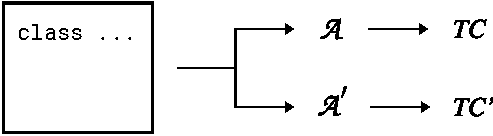
\includegraphics[width=0.6\linewidth]{figures/delta_test_coverage_approach}
  \caption{For each class, two test suites are generated, resulting in two activity matrices \(\mathcal{A} \) and \(\mathcal{A}' \). For each activity matrix, we compute test coverage \(TC \), DDU, normalized density, diversity, uniqueness.}%
  \label{fig:delta_test_coverage_approach}
\end{figure}

For the third experiment, we generate two test suites with different DDU values and investigate whether the error detection improves when DDU improves, as illustrated in \Cref{fig:delta_error_detection_approach}.
Similar to the first experiment, we generate 10 fault candidates of cardinality 2 and compute the error vector with an \emph{oracle probability} of 0.75 to determine the error detection.
To account for randomness of generating fault candidates, we repeat this process 10 times.
\begin{figure}
  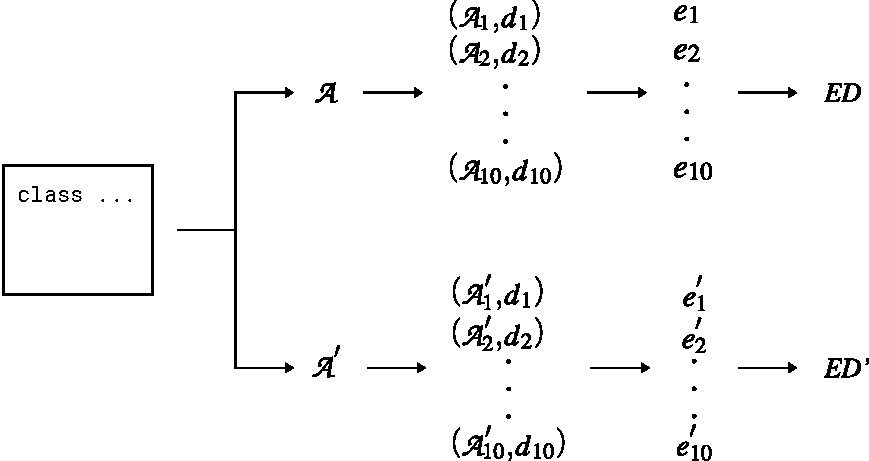
\includegraphics[width=\linewidth]{figures/delta_error_detection_approach}
  \caption{For each class, we generate two different test suites, resulting in two activity matrices. For each matrix, we generate 10 fault candidates of cardinality 2 and compute the error vector. Finally, we compute the error detection and repeat this process 10 times.}%
  \label{fig:delta_error_detection_approach}
\end{figure}

\section{Experimental Results}
In the first experiment, we confirm whether test coverage is representative for error detection.
In \Cref{fig:coverage_error_detection}, we observe that there is a strong correlation between branch coverage and error detection.
We can say with 95\% confidence that branch coverage is positively correlated with error detection.
Furthermore, we observe in \Cref{fig:coverage_error_detection} that all data points are in the lower right corner, meaning that branch coverage puts an upper bound on error detection.
The upper bound can be explained with the following example.
Assuming that 60\% of the components are tested, faults that involve untested components (in the remaining 40\%) can never be detected and, therefore, the error detection can at most be 60\%.
Likewise, the error detection can at most be 100\% if the test coverage is 100\%.
In \Cref{tab:hightclowed}, an example is given of a class with 100\% test coverage but 0\% error detection for faults of cardinality 2.
To summarize, the error detection for a class can at most be equal to the test coverage.
\begin{figure}
  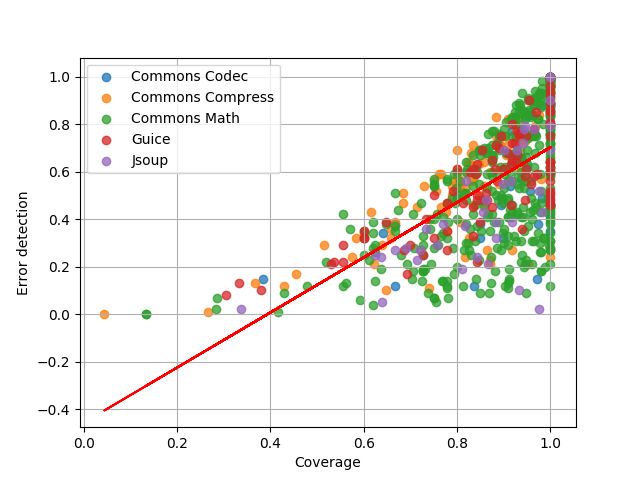
\includegraphics[width=\linewidth]{figures/coverage_error_detection}
  \caption{Scatterplot of coverage and error detection, \(r = 0.628 \), \(p < 0.01 \).}%
  \label{fig:coverage_error_detection}
\end{figure}

\begin{table}[]
    \centering
    \caption{Example of activity matrix with a high test coverage of 100\% but a low error detection for faults with a cardinality of two.}%
    \label{tab:hightclowed}
    \begin{tabular}{l|llll}
    transactions & \(c_1 \) & \(c_2 \) & \(c_3 \) & \(c_4 \) \\ \hline
    \(t_1 \) & 1 & 0 & 0 & 0 \\
    \(t_2 \) & 0 & 1 & 0 & 0 \\
    \(t_3 \) & 0 & 0 & 1 & 0 \\
    \(t_4 \) & 0 & 0 & 0 & 1
    \end{tabular}
\end{table}

In the second experiment, we examine the correlation between normalized density, diversity, uniqueness, and DDU on the one hand, and branch coverage on the other.
The results are shown in \Cref{fig:coverage_metric} and \Cref{fig:delta_coverage_metric}.
We observe in \Cref{fig:coverage_density} and \Cref{fig:coverage_diversity} that normalized density is uncorrelated to branch coverage, and that diversity is weakly correlated to branch coverage.
In \Cref{fig:coverage_uniqueness} and \Cref{fig:coverage_ddu}, we observe that uniqueness and DDU are weakly correlated to branch coverage.

Although uniqueness and DDU have a weak correlation with branch coverage, in \Cref{fig:coverage_uniqueness} and \Cref{fig:coverage_ddu}, we observe that uniqueness and DDU put a lower bound on branch coverage --- all data points are located in the upper left corner of the plot.
The branch coverage is lower bounded by uniqueness since uniqueness corresponds to the number of unique columns in the activity matrix.
This means that if the uniqueness is low, then the number of unique columns is low and therefore the branch coverage is potentially low.
In \Cref{subfig:low_uniqueness} and \Cref{subfig:low_uniqueness_high_coverage}, we provide examples illustrating how branch coverage can be high or low given an activity matrix with a low uniqueness.
If the uniqueness is high, then the number of unique columns is high and therefore the branch coverage has to be high too.
In \Cref{subfig:optimal_uniqueness_coverage} and \Cref{subfig:optimal_uniqueness}, we provide two activity matrices with optimal uniqueness, resulting in a relative high or optimal coverage.
Consequently, the DDU lower bounds branch coverage because uniqueness is a component of DDU\@.

Similar results are found in the experiment where an improvement in a diagnosability assessment metric is compared with a difference in test coverage, see \Cref{fig:delta_coverage_metric}.
In \Cref{fig:delta_coverage_density}, \Cref{fig:delta_coverage_diversity}, and \Cref{fig:delta_coverage_ddu}, we observe that an improvement in normalized density, diversity, and DDU is weakly correlated with an increase in branch coverage.
Also, an improvement in uniqueness is strongly correlated with an improvement in branch coverage, as illustrated in \Cref{fig:delta_coverage_uniqueness}, which could be related to our previous observation where uniqueness puts a lower bound on branch coverage.
However, DDU does not show similar results --- a strong correlation with an improvement in branch coverage, which could be caused by the fact that normalized density and diversity reduce the effect of uniqueness.


\begin{figure*}
    \centering
    \begin{subfigure}[b]{0.49\linewidth}
        \centering
        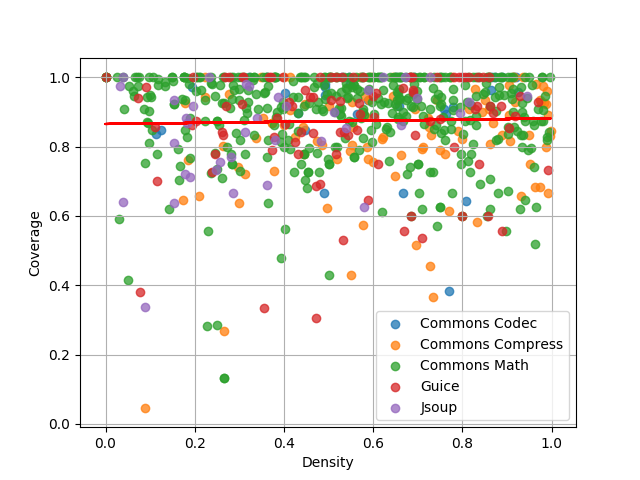
\includegraphics[width=\linewidth]{figures/coverage_density}
        \caption{Normalized density, \(r=0.029 \), \(p = 0.44 \).}%
        \label{fig:coverage_density}
    \end{subfigure}
    \hfill
    \begin{subfigure}[b]{0.49\linewidth}
        \centering
        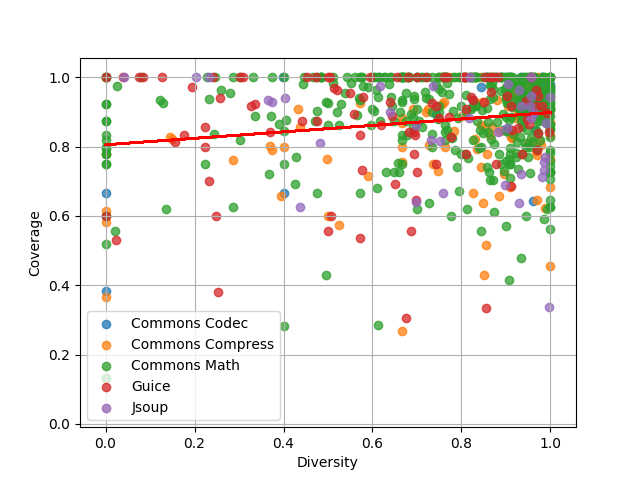
\includegraphics[width=\linewidth]{figures/coverage_diversity}
        \caption{Diversity, \(r=0.173 \), \(p < 0.01 \).}%
        \label{fig:coverage_diversity}
    \end{subfigure}
    \vskip\baselineskip%
    \begin{subfigure}[b]{0.49\linewidth}
        \centering
        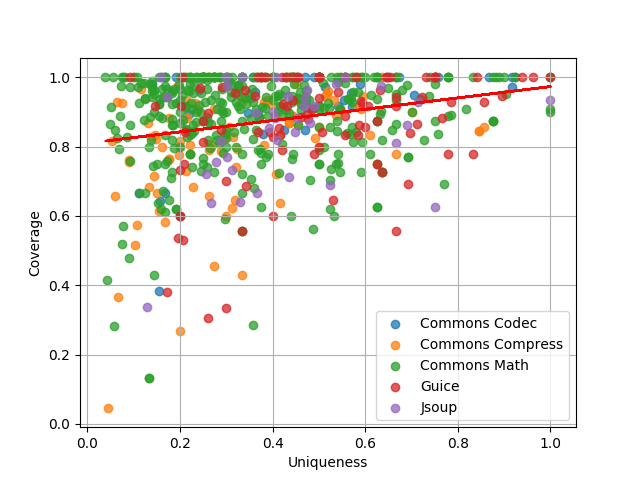
\includegraphics[width=\linewidth]{figures/coverage_uniqueness}
        \caption{Uniqueness, \(r=0.237 \), \(p<0.01 \).}%
        \label{fig:coverage_uniqueness}
    \end{subfigure}
    \hfill
    \begin{subfigure}[b]{0.49\linewidth}
        \centering
        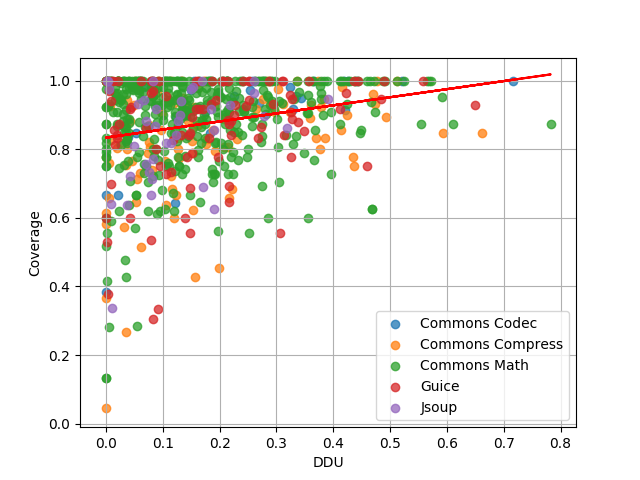
\includegraphics[width=\linewidth]{figures/coverage_ddu}
        \caption{DDU, \(r=0.228 \), \(p<0.01 \).}%
        \label{fig:coverage_ddu}
    \end{subfigure}
    \caption{Scatterplot of normalized density, diversity, uniqueness, and DDU against branch coverage.}%
    \label{fig:coverage_metric}
\end{figure*}

\begin{figure*}
    \centering
    \begin{subfigure}[b]{0.49\linewidth}
        \centering
        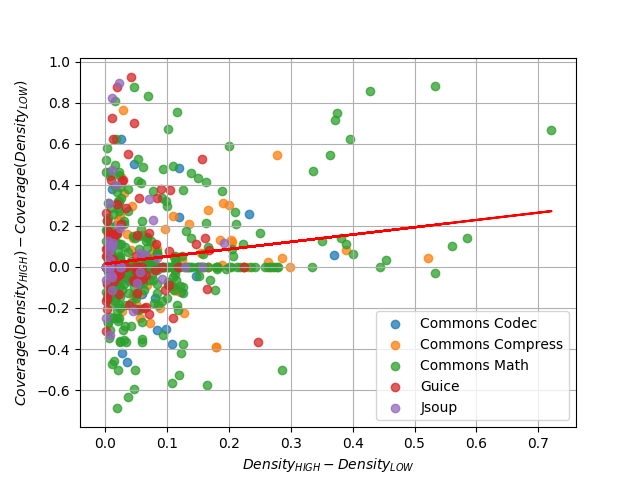
\includegraphics[width=\linewidth]{figures/delta_coverage_density}
        \caption{Normalized density, \(r=0.143 \), \(p<0.01 \).}%
        \label{fig:delta_coverage_density}
    \end{subfigure}
    \hfill
    \begin{subfigure}[b]{0.49\linewidth}
        \centering
        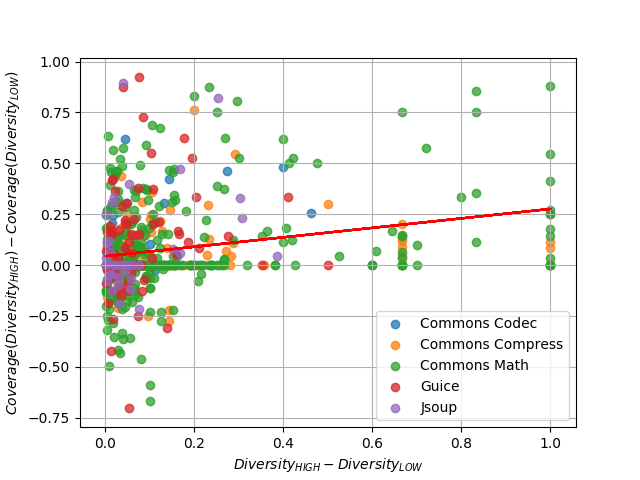
\includegraphics[width=\linewidth]{figures/delta_coverage_diversity}
        \caption{Diversity, \(r=0.230 \), \(p < 0.01 \).}%
        \label{fig:delta_coverage_diversity}
    \end{subfigure}
    \vskip\baselineskip%
    \begin{subfigure}[b]{0.49\linewidth}
        \centering
        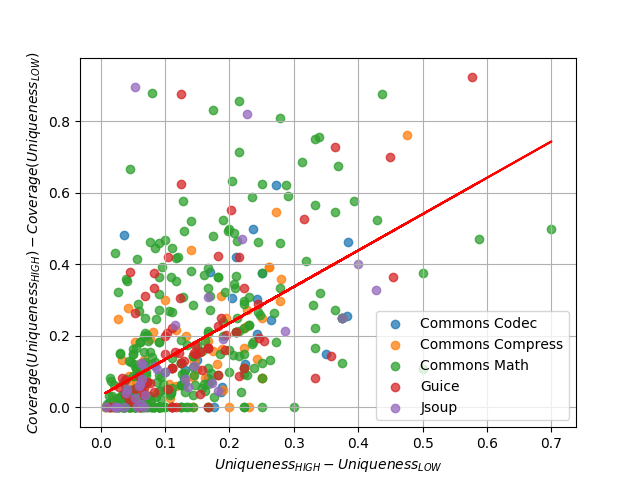
\includegraphics[width=\linewidth]{figures/delta_coverage_uniqueness}
        \caption{Uniqueness, \(r=0.546 \), \(p<0.01 \).}%
        \label{fig:delta_coverage_uniqueness}
    \end{subfigure}
    \hfill
    \begin{subfigure}[b]{0.49\linewidth}
        \centering
        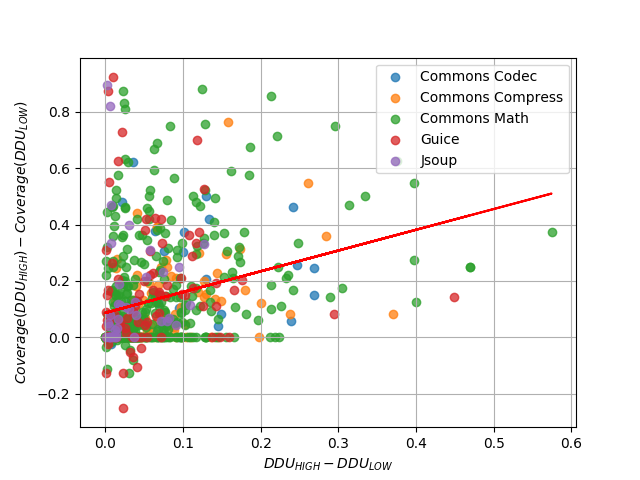
\includegraphics[width=\linewidth]{figures/delta_coverage_ddu}
        \caption{DDU, \(r=0.290 \), \(p<0.01 \).}%
        \label{fig:delta_coverage_ddu}
    \end{subfigure}
    \caption{Scatterplot of delta normalized density, delta diversity, delta uniqueness, and delta DDU against delta branch coverage.}%
    \label{fig:delta_coverage_metric}
\end{figure*}

\begin{figure*}
    \centering
    \begin{subfigure}[b]{0.48\linewidth}
        \centering
        \begin{tabular}{c|cccc}
          & \(c_1 \) & \(c_2 \) & \dots & \(c_{10} \)     \\ \hline
          \(t_1 \) & 1 & 0 & \dots & 0 \\
          \(t_2 \) & 1 & 0 & \dots & 0 \\
          \(t_3 \) & 1 & 0 & \dots & 0 \\
          \(t_4 \) & 1 & 0 & \dots & 0 \\
        \end{tabular}
        \caption{Low uniqueness, \(\mathcal{U}=0.2 \), \(coverage = 0.1 \).}%
        \label{subfig:low_uniqueness}
    \end{subfigure}
    \hfill
    \begin{subfigure}[b]{0.49\linewidth}
        \centering
        \begin{tabular}{c|cccc}
          & \(c_1 \) & \(c_2 \) & \dots & \(c_{10} \)     \\ \hline
          \(t_1 \) & 1 & 1 & \dots & 1 \\
          \(t_2 \) & 1 & 1 & \dots & 1 \\
          \(t_3 \) & 1 & 1 & \dots & 1 \\
          \(t_4 \) & 1 & 1 & \dots & 1 \\
        \end{tabular}
        \caption{Low uniqueness, \(\mathcal{U}=0.1 \), \(coverage = 1.0 \).}%
        \label{subfig:low_uniqueness_high_coverage}
    \end{subfigure}
    \vskip\baselineskip%
    \begin{subfigure}[b]{0.49\linewidth}
        \centering
        \begin{tabular}{c|cccc}
          & \(c_1 \) & \(c_2 \) & \(c_3 \) & \(c_4 \)     \\ \hline
          \(t_1 \) & 1 & 0 & 0 & 0 \\
          \(t_2 \) & 0 & 1 & 0 & 0 \\
          \(t_3 \) & 0 & 0 & 1 & 0 \\
          \(t_4 \) & 0 & 0 & 0 & 1 \\
        \end{tabular}
        \caption{Optimal uniqueness, \(\mathcal{U}=1.0 \), \(coverage = 1.0 \).}%
        \label{subfig:optimal_uniqueness_coverage}
    \end{subfigure}
    \hfill
    \begin{subfigure}[b]{0.49\linewidth}
        \centering
        \begin{tabular}{c|cccc}
          & \(c_1 \) & \(c_2 \) & \(c_3 \) & \(c_4 \)     \\ \hline
          \(t_1 \) & 1 & 0 & 0 & 0 \\
          \(t_2 \) & 0 & 1 & 0 & 0 \\
          \(t_3 \) & 0 & 0 & 1 & 0 \\
          \(t_4 \) & 0 & 0 & 0 & 0 \\
        \end{tabular}
        \caption{Optimal uniqueness, \(\mathcal{U}=1.0 \), \(coverage = 0.75 \).}%
        \label{subfig:optimal_uniqueness}
    \end{subfigure}
    \caption{Examples of activity matrices with a low or high uniqueness.}
\end{figure*}

In the third experiment, we analyze the relation between DDU and error detection.
In \Cref{fig:error_detection_metric}, we observe that there is no strong correlation between normalized density, diversity, uniqueness, and DDU on the one hand, and error detection on the other.
In \Cref{fig:delta_error_detection_metric}, we observe similar results; no strong correlation between delta normalized density, delta diversity, delta uniqueness, delta DDU, and delta error detection, i.e.\ improving a diagnosability assessment metric does not result in an improvement in error detection.
The results in \Cref{fig:error_detection_uniqueness} and \Cref{fig:delta_error_detection_uniqueness} are unexpected because we have seen in previous experiments that branch coverage is strongly correlated to error detection, see \Cref{fig:coverage_error_detection}, and that an improvement in uniqueness is strongly correlated to an improvement in branch coverage, see \Cref{fig:delta_coverage_uniqueness}.
However, we do not observe any correlation between uniqueness and error detection.

\begin{figure*}
    \centering
    \begin{subfigure}[b]{0.49\linewidth}
        \centering
        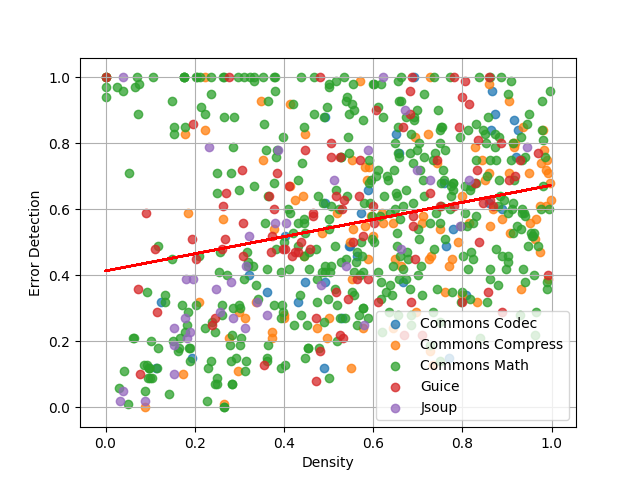
\includegraphics[width=\linewidth]{figures/error_detection_density}
        \caption{Normalized density, \(r=0.256 \), \(p<0.01 \).}%
        \label{fig:error_detection_density}
    \end{subfigure}
    \hfill
    \begin{subfigure}[b]{0.49\linewidth}
        \centering
        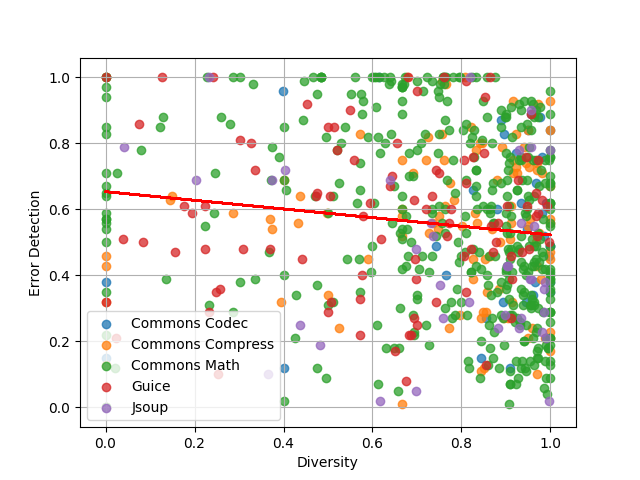
\includegraphics[width=\linewidth]{figures/error_detection_diversity}
        \caption{Diversity, \(r=-0.132 \), \(p < 0.01 \).}%
        \label{fig:error_detection_diversity}
    \end{subfigure}
    \vskip\baselineskip%
    \begin{subfigure}[b]{0.49\linewidth}
        \centering
        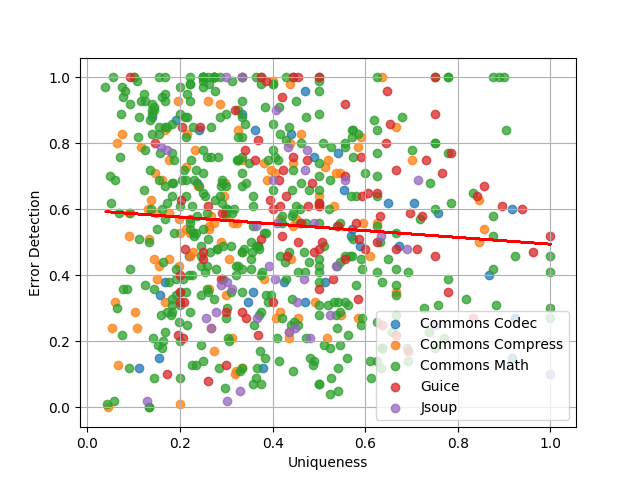
\includegraphics[width=\linewidth]{figures/error_detection_uniqueness}
        \caption{Uniqueness, \(r=-0.080 \), \(p<0.05 \).}%
        \label{fig:error_detection_uniqueness}
    \end{subfigure}
    \hfill
    \begin{subfigure}[b]{0.49\linewidth}
        \centering
        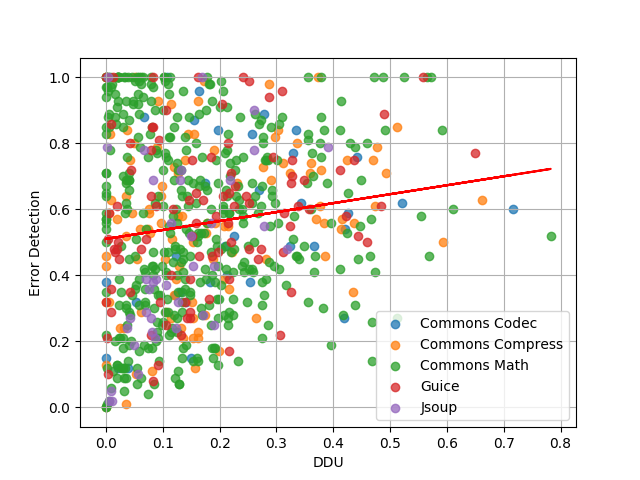
\includegraphics[width=\linewidth]{figures/error_detection_ddu}
        \caption{DDU, \(r=0.142 \), \(p<0.01 \).}%
        \label{fig:error_detection_ddu}
    \end{subfigure}
    \caption{Scatterplot of normalized density, diversity, uniqueness, and DDU against error detection.}%
    \label{fig:error_detection_metric}
\end{figure*}

\begin{figure*}
    \centering
    \begin{subfigure}[b]{0.49\linewidth}
        \centering
        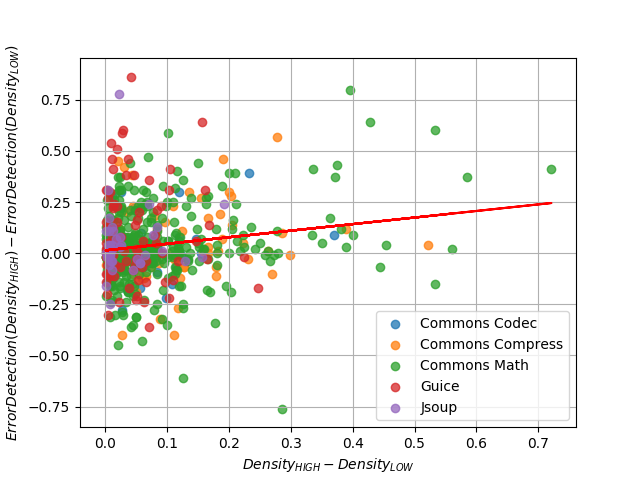
\includegraphics[width=\linewidth]{figures/delta_error_detection_density}
        \caption{Normalized density, \(r=0.165 \), \(p<0.01 \).}%
        \label{fig:delta_error_detection_density}
    \end{subfigure}
    \hfill
    \begin{subfigure}[b]{0.49\linewidth}
        \centering
        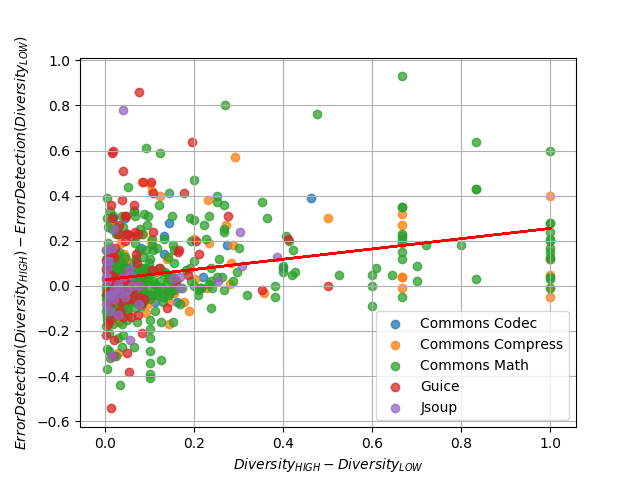
\includegraphics[width=\linewidth]{figures/delta_error_detection_diversity}
        \caption{Diversity, \(r=0.275 \), \(p < 0.01 \).}%
        \label{fig:delta_error_detection_diversity}
    \end{subfigure}
    \vskip\baselineskip%
    \begin{subfigure}[b]{0.49\linewidth}
        \centering
        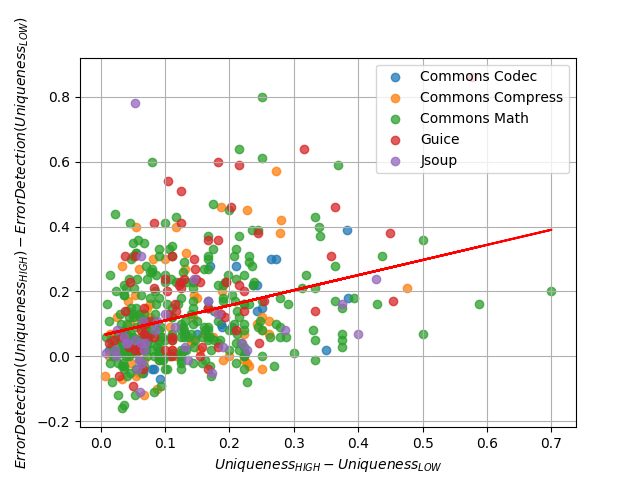
\includegraphics[width=\linewidth]{figures/delta_error_detection_uniqueness}
        \caption{Uniqueness, \(r=0.323 \), \(p<0.01 \).}%
        \label{fig:delta_error_detection_uniqueness}
    \end{subfigure}
    \hfill
    \begin{subfigure}[b]{0.49\linewidth}
        \centering
        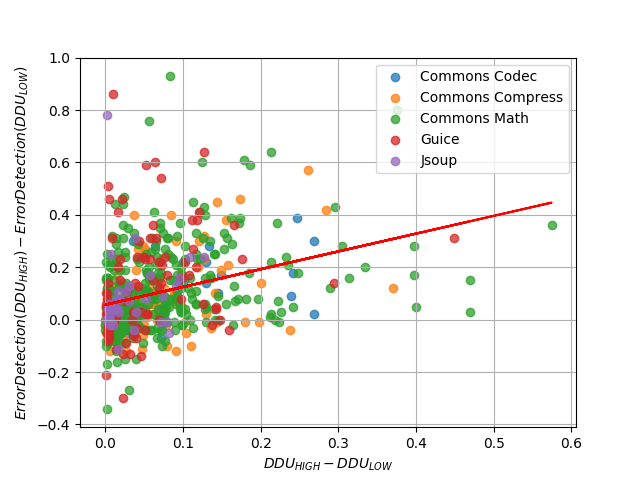
\includegraphics[width=\linewidth]{figures/delta_error_detection_ddu}
        \caption{DDU, \(r=0.324 \), \(p<0.01 \).}%
        \label{fig:delta_error_detection_ddu}
    \end{subfigure}
    \caption{Scatterplot of delta normalized density, delta diversity, delta uniqueness, and delta DDU against delta error detection.}%
    \label{fig:delta_error_detection_metric}
\end{figure*}

Revisiting the third research question:
\begin{framed}
\noindent
\textbf{RQ3:} What is the relation between density, diversity, uniqueness, and DDU and test coverage?
\end{framed}
\textbf{A:} In the first experiment, we confirmed that branch coverage is strongly correlated to error detection.
In the second experiment, in which we analyze the relation between the diagnosability metrics and branch coverage, we observed that only an improvement in uniqueness is strongly correlated to an improvement in branch coverage.
The other metrics did not show any significant correlation.
Further, we observed that uniqueness and DDU put a lower bound on branch coverage.
In final experiment, we found no evidence that uniqueness and the other diagnosability metrics are correlated to error detection.

\chapter{Conclusion}%
\label{ch:conclusion}

% Goal of this study
% Why is this important?

In this work, we performed the first study on DDU, a metric that quantifies the diagnosability of software systems, proposed by Perez \etal~\cite{DBLP:conf/icse/PerezAD17}.
The goal of this study was to obtain knowledge about DDU such that it can be made usable in practice as an aid to developers in writing better tests.
\emph{Better tests}, in this study, are defined as tests that can easily and precisely locate the root cause of a failure, also known as diagnosability.
A high diagnosability is important because it can potentially reduce the time spent on debugging, which currently accounts for 30\% to 90\% of the software development cycle.

% In prior work, Perez \etal~\cite{DBLP:conf/icse/PerezAD17} proposed DDU, a complementary metric to test coverage that measures the diagnosability of software systems.
% The authors find evidence that optimizing a test suite with respect to DDU yields a 34\% gain in diagnostic performance with spectrum-based reasoning compared to branch coverage.
% However, the problem with DDU is that it is not usable in practice due to its output value between 0 and 1.

% Therefore, we performed the first study on DDU\@.
% In this study, we explored the behavior of DDU in practice and investigated its correlation with diagnosability and test coverage to obtain insight in how DDU can be used in practice.

To better understand the capabilities of DDU, we answer the research questions defined in \Cref{ch:research_questions} by analyzing real-world code repositories, namely Commons Codec, Commons Compress, Commons Math, Guice and Jsoup.

\begin{framed}
\noindent
\textbf{RQ1:} How do normalized density, diversity, uniqueness, and DDU vary in practice?
\end{framed}

In \Cref{ch:rq1}, we explored the behavior of the diagnosability assessment metrics by analyzing existing software systems.
We looked at various activity matrices to see what influences the diagnosability assessment metrics to have a low or high value.
We found that DDU is right-tailed, that is, it is difficult to write tests to obtain an optimal DDU value of 1.

\begin{framed}
\noindent
\textbf{RQ2:} What is the relation between normalized density, diversity, uniqueness, and DDU and diagnosability?
\end{framed}

In \Cref{ch:rq2}, we performed experiments to investigate the relation between the diagnosability assessment metrics and diagnosability.
We found no strong evidence that DDU is correlated to diagnosability, measured in effort, although prior study~\cite{DBLP:conf/icse/PerezAD17} showed evidence that DDU improves the diagnosability when generating tests that are optimized with respect to DDU\@.
Therefore, this means that current tests written in open source projects, according to DDU, are not written with the intent to optimize diagnosability.

\begin{framed}
\noindent
\textbf{RQ3:} What is the relation between density, diversity, uniqueness, and DDU and test coverage?
\end{framed}

In \Cref{ch:rq3}, we performed experiments to investigate the relation between the diagnosability assessment metrics and test coverage to understand how DDU could potentially be used together with test coverage.
We found that normalized density, diversity, DDU have a weak correlation with test coverage, and that uniqueness is strongly correlated to test coverage.
However, uniqueness does not have a strong correlation with error detection, which is supposedly measured by test coverage.

\section{Future Work}
% The projects are well-tested, why do they not have a high diagnosability? How important is diagnosability in practice?
The experimental results have shown that DDU and its components do not have a strong correlation with diagnosability in practice.
Therefore, it is worth researching if manually writing tests to optimize diagnosability is useful in practice at all.
Also, we pose the question if diagnosability is only useful for automated debugging techniques because prior work~\cite{DBLP:conf/icse/PerezAD17} has shown that optimizing tests with respect to DDU when generating tests results in an increase in diagnosability.
To answer these questions, we propose a case study or user study in which a deeper understanding should be obtained on why developers write tests and to investigate whether developers desire tests that improve the diagnosability.
% Theoretically, writing tests that optimize diagnosability would be beneficial to automated debugging techniques, like spectrum-based reasoning, but we have seen in practice that barely any class has a high 

Furthermore, DDU is supposedly a metric that quantifies diagnosability, the property of faults to be easily and precisely located~\cite{730889}.
Currenlty, DDU is only useful when generating tests to increase the diagnostic performance of SBFL techniques.
However, Parnin and Orso~\cite{Parnin:2011:ADT:2001420.2001445} found evidence in a prelimenary user study that a high diagnostic performance does not result in a shorter debugging time due to the lack of context provided by SBFL techniques to understand the root cause.
Therefore, we pose the question: how important is diagnosability in practice?

We analyzed DDU due to its possibility to improve the diagnostic performance of automated debugging techniques.
However, there has been no study that investigates the impact of diagnosability on the debugging activity when performed by the developer without automated debugging techniques.
Future work could perform a user study with two developer groups, where one group tries to locate the fault with tests that are optimized for test coverage and the other group tries to locate the fault with tests that are optimized for diagnosability.

In this study, most experiments are performed by injecting faults of cardinality 2, which is similar to the cardinality used by prior work~\cite{DBLP:conf/icse/PerezAD17}.
However, Perez \etal~\cite{7927959} showed evidence with an empirical study that single-component faults are prevalent --- over 82\% of the bugs found in 279 open source projects involved a single-component fault.
This means that DDU can be modified to account for these findings, for example, by biasing DDU towards single-component faults.

% Is diagnosability only important for test generation?

% DDU seems to have no correlation with diagnosability in practice. How can DDU be modified

% 80% coverage then DDU

% future experiments

\bibliographystyle{plain}
\bibliography{bibliography}

\end{document}
